% !TEX program = xelatex
\documentclass[14pt,a4paper]{extarticle}

\usepackage{fontspec}
\usepackage{polyglossia}
\setdefaultlanguage{russian}
\setotherlanguage{english}
\IfFontExistsTF{Times New Roman}{%
    \setmainfont{Times New Roman}
    \newfontfamily\cyrillicfont{Times New Roman}[Script=Cyrillic]
}{%
    \IfFontExistsTF{Tinos}{%
        \setmainfont{Tinos}
        \newfontfamily\cyrillicfont{Tinos}[Script=Cyrillic]
    }{%
        \setmainfont{Liberation Serif}
        \newfontfamily\cyrillicfont{Liberation Serif}[Script=Cyrillic]
    }%
}%
\setmonofont{DejaVu Sans Mono}

\usepackage[a4paper,left=30mm,right=15mm,top=20mm,bottom=20mm]{geometry}
\usepackage{setspace}
\usepackage{indentfirst}
\usepackage{amsmath,amssymb}
\usepackage{graphicx}
\usepackage{float}
\usepackage{array}
\usepackage{longtable}
\usepackage{ragged2e}
\usepackage{booktabs}
\usepackage{caption}
\usepackage{hyperref}
\usepackage{xurl}
\usepackage{enumitem}
\usepackage{makecell}
\usepackage{multirow}
\usepackage{titlesec}
\usepackage{tocloft}
\usepackage{adjustbox}
\usepackage{needspace}
\usepackage{etoolbox}
\usepackage[section]{placeins}
\usepackage[most]{tcolorbox}
\usepackage{pdfpages}
\usepackage{atbegshi}
\AtBeginShipout{\special{pdf: put @thispage << /Rotate 0 >>}}

\hypersetup{hidelinks}
\pagestyle{plain}
\sloppy
\frenchspacing
\urlstyle{same}
\onehalfspacing
\setlength{\parindent}{1.25cm}
\setlength{\parskip}{0pt}

\setlength{\floatsep}{0.95\baselineskip}
\setlength{\textfloatsep}{1.05\baselineskip}
\setlength{\intextsep}{0.95\baselineskip}
\setlength{\LTpre}{0.65\baselineskip}
\setlength{\LTpost}{0.75\baselineskip}
\setlength{\abovecaptionskip}{0.45\baselineskip}
\setlength{\belowcaptionskip}{0.45\baselineskip}
\DeclareCaptionLabelSeparator{gost}{~—~}
\captionsetup{labelsep=gost, singlelinecheck=false, font=normalsize}
\captionsetup[table]{justification=raggedright, position=above, skip=0.45\baselineskip}
\captionsetup[figure]{justification=centering, skip=0.45\baselineskip}
\renewcommand{\arraystretch}{1.28}
\setlength{\tabcolsep}{4.4pt}
\setlength{\extrarowheight}{2.8pt}

\BeforeBeginEnvironment{table}{\par\vspace{0.35\baselineskip}\Needspace{8\baselineskip}}
\AfterEndEnvironment{table}{\vspace{0.45\baselineskip}}
\BeforeBeginEnvironment{figure}{\par\vspace{0.35\baselineskip}\Needspace{10\baselineskip}}
\AfterEndEnvironment{figure}{\vspace{0.55\baselineskip}}
\BeforeBeginEnvironment{longtable}{\par\vspace{0.25\baselineskip}\Needspace{8\baselineskip}}
\AfterEndEnvironment{longtable}{\vspace{0.55\baselineskip}}
\clubpenalty=10000
\widowpenalty=10000
\displaywidowpenalty=10000
\newcolumntype{L}[1]{>{\RaggedRight\arraybackslash}m{#1}}
\newcolumntype{C}[1]{>{\centering\arraybackslash}m{#1}}
\newcolumntype{R}[1]{>{\RaggedLeft\arraybackslash}m{#1}}
\setlength{\emergencystretch}{4em}
\setcounter{secnumdepth}{3}
\setcounter{tocdepth}{3}

\titleformat{\section}{\bfseries\normalsize}{\thesection}{0.9em}{}
\titleformat{\subsection}{\bfseries\normalsize}{\thesubsection}{0.6em}{}
\titleformat{\subsubsection}{\bfseries\normalsize}{\thesubsubsection}{0.6em}{}
\titlespacing*{\section}{1.25cm}{1.10\baselineskip}{0.85\baselineskip}
\titlespacing*{\subsection}{1.25cm}{1.00\baselineskip}{0.70\baselineskip}
\titlespacing*{\subsubsection}{1.25cm}{0.85\baselineskip}{0.55\baselineskip}

\renewcommand{\contentsname}{СОДЕРЖАНИЕ}
\renewcommand{\cftsecfont}{\normalfont}
\renewcommand{\cftsecpagefont}{\normalfont}

\newcommand{\pycmd}[1]{%
  \begin{tcolorbox}[enhanced,breakable,colback=white,colframe=black,boxrule=0.5pt,left=5pt,right=5pt,top=5pt,bottom=5pt,arc=0pt]
  {\ttfamily\small #1}
  \end{tcolorbox}%
}
\newcommand{\insertfig}[2][0.86\textwidth]{%
    \IfFileExists{#2}{\includegraphics[width=#1]{#2}}{%
        \fbox{\parbox[c][6cm][c]{0.8\textwidth}{\centering Файл изображения не найден:\ \texttt{\detokenize{#2}}}}%
    }%
}

\newcommand{\miniresult}[1]{%
    \par\vspace{0.30\baselineskip}%
    \noindent\textit{Вывод:} #1%
    \par\vspace{0.25\baselineskip}%
}

\newcommand{\structsection}[1]{%
    \clearpage\phantomsection%
    \begin{center}{\bfseries \MakeUppercase{#1}}\end{center}%
    \addcontentsline{toc}{section}{#1}%
}
\newcommand{\gostappendix}[2]{%
    \clearpage\phantomsection%
    \addcontentsline{toc}{section}{Приложение #1. #2}%
    \renewcommand{\thetable}{#1.\arabic{table}}%
    \renewcommand{\thefigure}{#1.\arabic{figure}}%
    \setcounter{table}{0}%
    \setcounter{figure}{0}%
    \begin{center}{\bfseries ПРИЛОЖЕНИЕ #1}\par\vspace{0.4\baselineskip}{\bfseries #2}\end{center}%
}

\newcommand{\NRespondents}{60}
\newcommand{\NObjects}{5}
\newcommand{\NGroups}{4}
\newcommand{\FemaleCount}{36}
\newcommand{\MaleCount}{24}
\newcommand{\UsedThreeMonthsCount}{57}
\newcommand{\MeanSpend}{3 002}
\newcommand{\MedianSpend}{1 950}
\newcommand{\FriedmanChi}{33,107}
\newcommand{\FriedmanP}{< 0,001}
\newcommand{\ConcordanceW}{0,138}
\newcommand{\FriedmanCleanChi}{30,202}
\newcommand{\FriedmanCleanP}{< 0,001}
\newcommand{\ConcordanceWClean}{0,132}
\newcommand{\ObjectFactorShare}{50,4}
\newcommand{\ExpertFactorShare}{64,8}
\newcommand{\RegRSq}{0,636}
\newcommand{\RegAdjRSq}{0,562}
\newcommand{\RegF}{8,579}
\newcommand{\RegFP}{< 0,001}

\begin{document}


\tableofcontents

\structsection{Введение}

Для студента сервис доставки — это не абстрактная цифровая платформа, а вполне практичный инструмент повседневной жизни. Один использует его, чтобы быстро перекусить между парами, другой — чтобы не тратить время на поход в магазин, третий — чтобы поймать выгодный промокод. Поэтому выбор сервиса складывается из нескольких мотивов сразу: цены, скорости, привычки к приложению и доверия к качеству.

В работе исследуется, как студенты воспринимают пять популярных сервисов доставки еды: Яндекс Еду, Самокат, Delivery Club, Купер и Ozon Fresh. Эти сервисы сравниваются по трем единым критериям — цене, скорости доставки и общему качеству, — а затем результаты дополняются анализом характеристик самих респондентов.

Цель работы состоит в объяснении логики различий в оценках сервисов, а не только в составлении итогового рейтинга. Для этого по данным опроса выполнены описательный анализ, факторный анализ объектов и характеристик экспертов, проверка согласованности мнений экспертной группы и регрессионное моделирование готовности рекомендовать сервис.

Исследование включало два связанных опроса. Первый опрос был посвящён базовой экспертной оценке сервисов по отдельным критериям. Во второй опрос были добавлены вопросы о характеристиках экспертов и факторах выбора: цене, скорости, скидках и промокодах, ассортименте, удобстве приложения, службе поддержки и точности времени доставки. В файле исходных данных эти части сохранены как листы \texttt{Опрос\_1} и \texttt{Опрос\_2}, а для анализа использован объединённый лист \texttt{Ответы\_объединенные}.

Опрос проведён онлайн среди студентов учебного потока 4414-4417. В итоговую таблицу вошло \NRespondents{} анкет, поэтому требование о количестве опрошенных не менее 30 человек выполнено. Оценивание проводилось по шкале от 1 до 10. В расчетах эта шкала трактуется как интервальная, что позволяет рассчитывать средние значения и ранги, применять факторный анализ, критерий Фридмана, коэффициент конкордации и регрессионную модель.

\clearpage
\section{Основная часть}

\subsection{Тема исследования и структура анкеты}

Тема исследования сформулирована как \textit{экспертная оценка сервисов доставки еды студентами}. Задача работы — не охватить весь рынок доставки и не объявить универсального победителя, а понять, как именно студенческая аудитория воспринимает разные сервисы. В фокусе находятся три вопроса: кто оказывается лидером по средним оценкам, какие скрытые факторы стоят за различиями между сервисами и насколько едино мнение респондентов.

Анкета состояла из трёх блоков:
\begin{enumerate}[leftmargin=1.25cm]
    \item профиль респондента: пол, возраст, учебная группа, частота использования доставки;
    \item оценки пяти сервисов по трём критериям: цена, скорость доставки, общее качество;
    \item характеристики эксперта: важность цены, скорости, скидок и промокодов, ассортимента, приложения, поддержки, точности времени доставки, месячные расходы, готовность рекомендовать сервис и привычка сравнивать цены.
\end{enumerate}

Первый блок описывает профиль эксперта, второй формирует матрицу оценок объектов, а третий позволяет связать оценки с поведением респондентов.

\subsection{Предобработка данных}

Исходный файл содержал \NRespondents{} строк ответов и не имел пропусков в ключевых вопросах. Перед расчётами данные были аккуратно подготовлены к статистическому анализу:
\begin{enumerate}[leftmargin=1.25cm]
    \item для каждого сервиса рассчитана интегральная оценка как среднее арифметическое трёх оценок: цены, скорости и общего качества;
    \item категориальные ответы о частоте использования и сравнении цен переведены в порядковые числовые шкалы;
    \item месячные расходы преобразованы через $\ln(1+x)$ для регрессионного анализа, поскольку распределение расходов имеет длинный правый хвост;
    \item отдельно отмечены кандидаты на удаление для проверки устойчивости согласованности экспертов: это респонденты, которые указали, что не пользуются доставкой, но при этом выставили оценки всем сервисам.
\end{enumerate}

Интегральная оценка объекта рассчитывалась по формуле
\begin{equation}
S_{ij}=\frac{x_{ij}^{price}+x_{ij}^{speed}+x_{ij}^{quality}}{3},
\end{equation}
где $S_{ij}$ - итоговая оценка $j$-го сервиса $i$-м экспертом, а три слагаемых соответствуют оценкам цены, скорости доставки и общего качества.

\subsection{Описание полученных результатов}

В выборке \FemaleCount{} респондентов указали женский пол, \MaleCount{} — мужской. По возрасту группа почти однородна: в ответах представлены в основном студенты 19 и 20 лет. За последние три месяца сервисами доставки пользовались \UsedThreeMonthsCount{} человек, то есть тема действительно знакома большинству участников на основе личного опыта. Средние месячные расходы составили около \MeanSpend{} рублей, а медианные — \MedianSpend{} рублей. Это различие показывает, что в выборке есть небольшая группа особенно активных пользователей, которая заметно повышает среднее значение.

Сводное распределение по ключевым категориальным вопросам приведено ниже.

\vspace{0.3\baselineskip}
{%
\small
\setlength{\tabcolsep}{3.2pt}
\renewcommand{\arraystretch}{1.08}
\begin{longtable}{L{4.1cm}L{5.2cm}R{1.1cm}R{1.3cm}}
\caption{Распределение ответов по ключевым вопросам анкеты}\label{tab:demographics}\\
\toprule
Блок & Категория & n & \% \\
\midrule
\endfirsthead
\toprule
Блок & Категория & n & \% \\
\midrule
\endhead
\midrule
\multicolumn{4}{r}{Продолжение на следующей странице}\\
\endfoot
\bottomrule
\endlastfoot
Пол & Женский & 36 & 60,0 \\
Пол & Мужской & 24 & 40,0 \\
Возраст & 19 & 31 & 51,7 \\
Возраст & 20 & 29 & 48,3 \\
Группа & 4414 & 13 & 21,7 \\
Группа & 4415 & 13 & 21,7 \\
Группа & 4416 & 23 & 38,3 \\
Группа & 4417 & 11 & 18,3 \\
Частота использования & 1 раз в неделю & 19 & 31,7 \\
Частота использования & 1-2 раза в месяц & 17 & 28,3 \\
Частота использования & Реже 1 раза в месяц & 9 & 15,0 \\
Частота использования & 2-3 раза в неделю & 8 & 13,3 \\
Частота использования & Почти каждый день & 4 & 6,7 \\
Частота использования & Не пользуюсь & 3 & 5,0 \\
Чаще используемый сервис & Яндекс Еда & 24 & 40,0 \\
Чаще используемый сервис & Самокат & 18 & 30,0 \\
Чаще используемый сервис & Ozon Fresh & 6 & 10,0 \\
Чаще используемый сервис & Купер & 5 & 8,3 \\
Чаще используемый сервис & Не пользуюсь & 3 & 5,0 \\
Чаще используемый сервис & Delivery Club & 3 & 5,0 \\
Чаще используемый сервис & Другой/локальный сервис & 1 & 1,7 \\
Сравнение цен & Иногда & 19 & 31,7 \\
Сравнение цен & Редко & 16 & 26,7 \\
Сравнение цен & Часто & 14 & 23,3 \\
Сравнение цен & Всегда & 7 & 11,7 \\
Сравнение цен & Никогда & 4 & 6,7 \\
\end{longtable}
}
\miniresult{выборка однородна по возрасту, но различается по опыту использования доставки. Поэтому оценки отражают взгляды студентов с разной частотой заказов, бюджетом и привычками выбора.}

Для оценок сервисов построена таблица средних значений. В ней отдельно показаны оценки по трём критериям, интегральная оценка и средний ранг сервиса в индивидуальных ранжировках экспертов.

\begin{table}[H]
\centering
\caption{Сводные показатели по оцениваемым сервисам}
\label{tab:service_summary}
{%
\small
\setlength{\tabcolsep}{3.0pt}
\renewcommand{\arraystretch}{1.12}
\begin{adjustbox}{max width=\textwidth}
\begin{tabular}{lrrrrrr}
\toprule
Сервис & Цена & Скорость & Качество & Средняя оценка & s & Средний ранг \\
\midrule
Самокат & 6,63 & 8,57 & 7,52 & 7,57 & 0,66 & 3,77 \\
Яндекс Еда & 6,68 & 7,45 & 7,95 & 7,36 & 0,67 & 3,41 \\
Delivery Club & 6,77 & 7,02 & 7,13 & 6,97 & 0,81 & 2,77 \\
Ozon Fresh & 7,32 & 6,50 & 6,90 & 6,91 & 0,83 & 2,62 \\
Купер & 7,10 & 6,63 & 6,80 & 6,84 & 0,68 & 2,42 \\
\bottomrule
\end{tabular}
\end{adjustbox}
}
\end{table}
\miniresult{Самокат лидирует по интегральной оценке, но отдельные критерии распределены между сервисами неравномерно. Поэтому рейтинг средних баллов полезен как отправная точка, но не объясняет всю структуру предпочтений. В таблице $s$ обозначает стандартное отклонение интегральных оценок сервиса.}

Уже на уровне средних видно, что сервисы воспринимаются по-разному: Самокат лучше других ассоциируется с быстрой доставкой, Яндекс Еда — с общим качеством, а Ozon Fresh — с более привлекательной ценой. Значит, одна итоговая оценка не может полностью описать картину.

\begin{figure}[H]
    \centering
    \insertfig[0.92\textwidth]{assets/favorite_service_bar.png}
    \caption{Распределение ответов на вопрос о чаще используемом сервисе}
    \label{fig:fav}
\end{figure}
\miniresult{чаще всего в выборке используют Яндекс Еду и Самокат. Значит, дальнейшие оценки отражают не только абстрактное восприятие брендов, но и реальный опыт взаимодействия с двумя наиболее привычными сервисами.}

\begin{figure}[H]
    \centering
    \insertfig[0.92\textwidth]{assets/service_criteria_grouped_bar.png}
    \caption{Средние оценки сервисов по критериям}
    \label{fig:criteria_bar}
\end{figure}
\miniresult{сервисы имеют разные сильные стороны: Самокат заметнее по скорости, Яндекс Еда — по качеству, Ozon Fresh — по цене. Поэтому итоговый рейтинг нужно читать вместе с отдельными критериями.}

\begin{figure}[H]
    \centering
    \insertfig[0.92\textwidth]{assets/service_criteria_heatmap_annotated.png}
    \caption{Тепловая карта средних оценок сервисов с выделением максимумов по критериям}
    \label{fig:heatmap}
\end{figure}
\miniresult{единого лидера по всем критериям нет: максимальная оценка цены у Ozon Fresh, скорости — у Самоката, качества — у Яндекс Еды. Следовательно, «лучший» сервис зависит от конкретного сценария выбора.}

Диаграмма и тепловая карта показывают, что оценки не сводятся к одной шкале «лучше-хуже»: у Самоката наиболее заметна скорость, у Яндекс Еды — качество, у Ozon Fresh — цена. Поэтому далее факторный анализ используется как разведочный инструмент, который помогает описать возможные скрытые направления различий.

\FloatBarrier
\subsection{Факторный анализ оцениваемых объектов}

В этом разделе сервисы рассматриваются не как набор отдельных средних оценок, а как система связанных мнений. Для каждого респондента была взята строка из пяти интегральных оценок, после чего оценки по каждому сервису стандартизированы:
\begin{equation}
z_{ij}=\frac{x_{ij}-\overline{x}_j}{s_j}.
\end{equation}

Стандартизация приводит оценки сервисов к одному масштабу. В качестве способа факторного анализа использован метод главных компонент, после выделения компонент применено varimax-вращение. Количество факторов выбрано по правилу собственных значений больше единицы. В компактной записи модель имеет вид
\begin{equation}
Z=FL^{T}+E,
\end{equation}
где $L$ показывает, с какими скрытыми факторами сильнее связан каждый сервис.

Перед интерпретацией факторов проверена пригодность данных для такого анализа. По оценкам сервисов тест Бартлетта не подтверждает статистически значимые связи между переменными, поэтому пригодность данных для факторного анализа объектов низкая. В связи с этим факторный анализ сервисов используется только как разведочная визуализация структуры оценок: он помогает компактно описать возможные направления различий, но не доказывает существование устойчивых типов восприятия или рыночных сегментов.

\begin{table}[H]
\centering
\caption{Проверка пригодности данных для факторного анализа}
\label{tab:factor_suitability}
{%
\small
\setlength{\tabcolsep}{3.0pt}
\renewcommand{\arraystretch}{1.15}
\begin{adjustbox}{max width=\textwidth}
\begin{tabular}{L{4.2cm}C{1.7cm}C{2.2cm}C{1.6cm}L{5.2cm}}
\toprule
Блок анализа & KMO & Bartlett $\chi^2$ & p-value & Вывод \\
\midrule
Оценки сервисов & 0,519 & 8,95 & 0,537 & Пригодность низкая: Bartlett p-value = 0,537 не подтверждает значимые связи; факторная карта используется только как разведочная визуализация. \\
Характеристики экспертов & 0,535 & 337,74 & < 0,001 & Пригодность также пограничная по KMO, но тест Бартлетта подтверждает наличие связей между признаками. \\
\bottomrule
\end{tabular}
\end{adjustbox}
}
\end{table}
\miniresult{для оценок сервисов KMO находится на нижней границе, а p-value Бартлетта равно 0,537, поэтому пригодность данных низкая. Ниже факторная карта используется только как разведочное описание структуры оценок; названия факторов являются условными интерпретациями. Для характеристик экспертов тест Бартлетта значим, но KMO также пограничный, поэтому выводы по факторам формулируются осторожно.}

\begin{table}[H]
\centering
\caption{Собственные значения факторов для оцениваемых объектов}
\label{tab:object_eigen}
{%
\small
\setlength{\tabcolsep}{3.0pt}
\renewcommand{\arraystretch}{1.12}
\begin{adjustbox}{max width=\textwidth}
\begin{tabular}{lrrr}
\toprule
Фактор & Собственное значение & Доля, \% & Накопл., \% \\
\midrule
F1 & 1,432 & 28,2 & 28,2 \\
F2 & 1,128 & 22,2 & 50,4 \\
F3 & 0,976 & 19,2 & 69,5 \\
F4 & 0,878 & 17,3 & 86,8 \\
F5 & 0,670 & 13,2 & 100,0 \\
\bottomrule
\end{tabular}
\end{adjustbox}
}
\end{table}
\miniresult{по правилу собственных значений больше единицы оставлены два фактора. Они объясняют около половины дисперсии, поэтому факторная карта является компактным, но неполным описанием различий между сервисами.}

\begin{table}[H]
\centering
\caption{Факторные нагрузки оцениваемых объектов после varimax-вращения}
\label{tab:object_loadings}
{%
\small
\setlength{\tabcolsep}{3.0pt}
\renewcommand{\arraystretch}{1.12}
\begin{adjustbox}{max width=\textwidth}
\begin{tabular}{lrrr}
\toprule
Сервис & F1 & F2 & h² \\
\midrule
Яндекс Еда & 0,253 & -0,604 & 0,430 \\
Самокат & 0,781 & 0,054 & 0,613 \\
Delivery Club & 0,471 & 0,458 & 0,431 \\
Купер & -0,001 & 0,715 & 0,511 \\
Ozon Fresh & 0,723 & -0,232 & 0,576 \\
\bottomrule
\end{tabular}
\end{adjustbox}
}
\end{table}
\miniresult{при интерпретации важны величины и знаки нагрузок. Чем больше абсолютная нагрузка, тем сильнее объект связан с соответствующим фактором.}

\begin{table}[H]
\centering
\caption{Содержательная интерпретация факторов оцениваемых объектов}
\label{tab:factor_interpretation}
{\small
\setlength{\tabcolsep}{3.0pt}
\renewcommand{\arraystretch}{1.18}
\begin{tabular}{L{2.1cm}C{2.0cm}L{4.1cm}L{6.0cm}}
\toprule
Фактор & Доля дисперсии & Сильные нагрузки & Осторожная интерпретация \\
\midrule
F1 & 28{,}2\% & Самокат (0{,}78), Ozon Fresh (0{,}72) & Фактор можно условно связать с практичным сценарием заказа: скорость и воспринимаемая выгодность. \\
F2 & 22{,}2\% & Купер (0{,}71), Delivery Club (0{,}46), Яндекс Еда (-0{,}60) & Фактор можно условно трактовать как альтернативное направление восприятия сервисов, отличающееся от позиции Яндекс Еды. \\
\bottomrule
\end{tabular}}
\end{table}
\miniresult{более сильным является F1: он объясняет 28,2\% дисперсии против 22,2\% у F2. С учётом слабой пригодности данных эти связи следует читать осторожно: на F1 сильнее всего нагружаются Самокат и Ozon Fresh, на F2 — Купер и Delivery Club, а Яндекс Еда имеет противоположный знак по F2.}

\begin{figure}[H]
    \centering
    \insertfig[0.84\textwidth]{assets/object_factor_importance.png}
    \caption{Вклад факторов в объяснение различий между оцениваемыми сервисами}
    \label{fig:object_factor_importance}
\end{figure}
\miniresult{F1 вносит больший вклад, чем F2, однако вместе два фактора объясняют только около половины различий между сервисами. Поэтому факторная модель показывает основные направления восприятия, но не исчерпывает всю структуру оценок.}

Первый фактор сильнее всего связан с Самокатом и Ozon Fresh. Его можно условно интерпретировать как \textit{практичный сценарий заказа}: в этой выборке он отражает повседневную полезность сервиса в ситуациях, где важны скорость и ощущение разумной цены. Второй фактор, по нагрузкам, условно формируется прежде всего Купером и Delivery Club и противопоставляется Яндекс Еде. Это не означает, что Яндекс Еда оценивается хуже: речь идёт о другом типе восприятия сервиса внутри общей структуры оценок.

\begin{figure}[H]
    \centering
    \insertfig[0.74\textwidth]{assets/object_factor_map_annotated.png}
    \caption{Карта факторных нагрузок оцениваемых объектов}
    \label{fig:object_factor_map}
\end{figure}
\miniresult{карта показывает не строго доказанные сегменты рынка, а возможные различия восприятия сервисов. Из-за слабой пригодности данных её следует трактовать как разведочную визуализацию.}

\FloatBarrier
\subsection{Факторный анализ характеристик экспертов}

Вторая часть факторного анализа относится не к сервисам, а к характеристикам самих экспертов. В расчёты включены вопросы о важности факторов выбора, частоте заказов, расходах, готовности рекомендовать сервис и сравнении цен. Часть ответов была изначально числовой, а порядковые категории были закодированы по смыслу: например, ответ «Не пользуюсь» получил значение 0, а «Почти каждый день» - значение 5.

\begin{table}[H]
\centering
\caption{Собственные значения факторов для характеристик экспертов}
\label{tab:expert_eigen}
{%
\small
\setlength{\tabcolsep}{3.0pt}
\renewcommand{\arraystretch}{1.12}
\begin{adjustbox}{max width=\textwidth}
\begin{tabular}{lrrr}
\toprule
Фактор & Собственное значение & Доля, \% & Накопл., \% \\
\midrule
F1 & 3,682 & 30,2 & 30,2 \\
F2 & 1,602 & 13,1 & 43,3 \\
F3 & 1,532 & 12,6 & 55,9 \\
F4 & 1,096 & 9,0 & 64,8 \\
F5 & 0,896 & 7,3 & 72,2 \\
F6 & 0,861 & 7,1 & 79,2 \\
\bottomrule
\end{tabular}
\end{adjustbox}
}
\end{table}
\miniresult{характеристики экспертов имеют более сложную структуру, чем оценки сервисов: выделяются четыре направления, связанные с частотой заказов, бюджетом, чувствительностью к цене и требованиями к качеству сервиса.}

По правилу собственных значений больше единицы оставлены четыре фактора. Вместе они объясняют \ExpertFactorShare{}\% дисперсии. Нагрузки после varimax-вращения приведены в таблице ниже.

\vspace{0.3\baselineskip}
{%
\small
\setlength{\tabcolsep}{3.2pt}
\renewcommand{\arraystretch}{1.08}
\begin{longtable}{L{5.2cm}R{1.35cm}R{1.35cm}R{1.35cm}R{1.35cm}R{1.2cm}}
\caption{Факторные нагрузки характеристик экспертов после varimax-вращения}\label{tab:expert_loadings}\\
\toprule
Переменная & F1 & F2 & F3 & F4 & h² \\
\midrule
\endfirsthead
\toprule
Переменная & F1 & F2 & F3 & F4 & h² \\
\midrule
\endhead
\midrule
\multicolumn{6}{r}{Продолжение на следующей странице}\\
\endfoot
\bottomrule
\endlastfoot
важность цены & -0,016 & -0,053 & 0,847 & -0,047 & 0,723 \\
важность скорости & 0,287 & 0,640 & 0,073 & 0,039 & 0,499 \\
важность скидок & 0,260 & -0,502 & 0,445 & -0,026 & 0,519 \\
важность ассортимента & 0,018 & 0,756 & -0,065 & -0,106 & 0,588 \\
важность приложения & -0,190 & 0,108 & 0,610 & 0,229 & 0,472 \\
важность поддержки & 0,177 & -0,338 & -0,186 & -0,704 & 0,676 \\
точность времени & 0,198 & -0,273 & -0,098 & 0,794 & 0,754 \\
частота заказов & 0,820 & 0,132 & 0,124 & 0,046 & 0,707 \\
расходы (log) & 0,962 & 0,012 & 0,032 & 0,046 & 0,928 \\
готовность рекомендовать & 0,838 & -0,004 & -0,253 & -0,096 & 0,775 \\
сравнение цен & 0,599 & 0,383 & 0,095 & 0,071 & 0,519 \\
пользовался 3 мес. & 0,859 & -0,089 & -0,058 & 0,035 & 0,751 \\
\end{longtable}
}
\miniresult{расхождения в оценках связаны не только с самими сервисами, но и с тем, насколько доставка встроена в повседневную жизнь респондента.}

Первый фактор имеет высокие положительные нагрузки по частоте заказов, расходам, факту использования доставки за последние три месяца и готовности рекомендовать сервис. В факторном анализе готовность рекомендовать рассматривается как поведенческий показатель респондента, а в регрессионной модели — как целевая переменная; эти два блока анализа решают разные задачи. В рамках разведочной интерпретации первый фактор удобно назвать фактором \textit{вовлечённости в доставку}: он показывает, насколько доставка встроена в повседневную жизнь студента.

Второй фактор связан с важностью скорости и ассортимента — это сценарий, в котором сервис ценят за оперативность и широту выбора. Третий фактор объединяет цену, скидки и удобство приложения: здесь на первый план выходит рациональный и выгодный заказ. Четвёртый фактор задаётся точностью времени доставки и службой поддержки и отражает ожидание предсказуемого сервиса без сбоев. В сумме эти факторы показывают, что различия в оценках связаны не только с самими платформами, но и с образом использования доставки у разных студентов.

\begin{figure}[H]
    \centering
    \insertfig[0.90\textwidth]{assets/expert_factor_loadings_heatmap.png}
    \caption{Факторные нагрузки характеристик экспертов}
    \label{fig:expert_heatmap}
\end{figure}
\miniresult{главный фактор экспертов — вовлеченность в доставку: он связан с расходами, частотой заказов, недавним использованием и готовностью рекомендовать сервис. Именно этот фактор объясняет наибольшую долю различий между респондентами.}

\begin{figure}[H]
    \centering
    \insertfig[0.96\textwidth]{assets/expert_factor_top_loadings.png}
    \caption{Наиболее сильные признаки в каждом факторе характеристик экспертов}
    \label{fig:expert_top_loadings}
\end{figure}
\miniresult{F1 отвечает за вовлеченность и объясняет 30,2\% дисперсии; F2 — за скорость и ассортимент; F3 — за цену, скидки и приложение; F4 — за точность времени доставки и поддержку. Так видно, какие признаки сильнее всего формируют каждый фактор.}

\FloatBarrier
\subsection{Оценка согласованности экспертов}

Для оценки согласованности использовались интегральные оценки пяти сервисов. Сначала для каждого респондента сервисы были проранжированы от наименее высокой к наиболее высокой оценке. Затем применён критерий Фридмана, который проверяет, можно ли считать различия между связанными ранговыми выборками случайными.

Нулевая гипотеза:
\begin{equation*}
H_0: \text{распределения оценок пяти сервисов одинаковы.}
\end{equation*}
Альтернативная гипотеза:
\begin{equation*}
H_1: \text{хотя бы один сервис отличается по оценкам экспертов.}
\end{equation*}

Статистика критерия Фридмана рассчитывается по формуле
\begin{equation}
\chi_F^2=\frac{12}{nk(k+1)}\sum_{j=1}^{k}R_j^2-3n(k+1),
\end{equation}
где $n$ - число экспертов, $k$ - число объектов, $R_j$ - сумма рангов $j$-го объекта.

Коэффициент конкордации Кендалла для случая без дополнительной поправки записан как
\begin{equation}
W=\frac{\chi_F^2}{n(k-1)}.
\end{equation}
Он принимает значения от 0 до 1: чем ближе $W$ к 1, тем выше согласованность экспертов.

\begin{table}[H]
\centering
\caption{Результаты критерия Фридмана и коэффициента конкордации}
\label{tab:friedman}
{%
\small
\setlength{\tabcolsep}{3.0pt}
\renewcommand{\arraystretch}{1.12}
\begin{adjustbox}{max width=\textwidth}
\begin{tabular}{lrrrr}
\toprule
Вариант расчёта & n & chi2\_F & p-value & W \\
\midrule
До удаления кандидатов & 60 & 33,107 & < 0,001 & 0,138 \\
После удаления кандидатов & 57 & 30,202 & < 0,001 & 0,132 \\
\bottomrule
\end{tabular}
\end{adjustbox}
}
\end{table}
\miniresult{различия между сервисами статистически значимы, но уровень единодушия в экспертной группе невысок. Иными словами, сервисы действительно различаются, однако респонденты не выстраивают их в полностью одинаковом порядке.}

Так как p-value меньше 0,001, нулевая гипотеза отвергается: сервисы действительно различаются статистически значимо. Однако коэффициент конкордации \ConcordanceW{} невысок. Это означает, что общее различие между сервисами есть, но единого «общестуденческого» порядка предпочтений не наблюдается: каждый респондент ранжирует сервисы немного по-своему.

Чтобы уточнить, какие именно пары сервисов различаются после общего теста Фридмана, дополнительно выполнены парные сравнения Уилкоксона для связанных выборок. Поскольку проверяется несколько пар одновременно, p-value скорректированы методом Холма. Такая проверка является пост-хок анализом: она не заменяет общий критерий Фридмана, а показывает, какие различия вносят основной вклад в общий результат.

\begin{table}[H]
\centering
\caption{Пост-хок сравнения сервисов: критерий Уилкоксона с поправкой Холма}
\label{tab:posthoc_wilcoxon}
{%
\small
\setlength{\tabcolsep}{3.0pt}
\renewcommand{\arraystretch}{1.10}
\begin{adjustbox}{max width=\textwidth}
\begin{tabular}{L{5.4cm}R{2.4cm}R{1.5cm}R{2.1cm}C{1.6cm}}
\toprule
Пара сервисов & Средняя разница & W & p Холма & Значимо \\
\midrule
Самокат — Купер & 0,728 & 160,0 & < 0,001 & да \\
Самокат — Ozon Fresh & 0,667 & 214,5 & < 0,001 & да \\
Самокат — Delivery Club & 0,600 & 272,0 & < 0,001 & да \\
Яндекс Еда — Купер & 0,517 & 322,5 & 0,002 & да \\
Яндекс Еда — Ozon Fresh & 0,456 & 377,0 & 0,010 & да \\
Яндекс Еда — Delivery Club & 0,389 & 433,0 & 0,096 & нет \\
Яндекс Еда — Самокат & -0,211 & 531,5 & 0,410 & нет \\
Delivery Club — Купер & 0,128 & 610,5 & 0,761 & нет \\
Delivery Club — Ozon Fresh & 0,067 & 629,5 & 0,891 & нет \\
Купер — Ozon Fresh & -0,061 & 643,0 & 0,891 & нет \\
\bottomrule
\end{tabular}
\end{adjustbox}
}
\end{table}
\miniresult{после поправки Холма Самокат значимо выше Delivery Club, Купера и Ozon Fresh. Яндекс Еда значимо выше Купера и Ozon Fresh, но отличие между Яндекс Едой и Самокатом статистически не подтверждается. Поэтому лидерство Самоката следует читать аккуратно: оно выражено в средних рангах, но не образует значимого отрыва от Яндекс Еды.}

Рейтинг сервисов следует трактовать как усреднённую тенденцию, а не как согласованный экспертный консенсус. Такой результат логичен для потребительской темы: студенты могут одинаково различать сервисы, но выбирать их по разным личным сценариям.

\begin{table}[H]
\centering
\caption{Средние ранги сервисов до и после удаления кандидатов}
\label{tab:mean_ranks}
{%
\small
\setlength{\tabcolsep}{3.0pt}
\renewcommand{\arraystretch}{1.12}
\begin{adjustbox}{max width=\textwidth}
\begin{tabular}{lrr}
\toprule
Сервис & Средний ранг & Средний ранг без кандидатов \\
\midrule
Яндекс Еда & 3,408 & 3,368 \\
Самокат & 3,775 & 3,781 \\
Delivery Club & 2,775 & 2,781 \\
Купер & 2,425 & 2,447 \\
Ozon Fresh & 2,617 & 2,623 \\
\bottomrule
\end{tabular}
\end{adjustbox}
}
\end{table}
\miniresult{после исключения формально сомнительных анкет порядок сервисов почти не меняется. Следовательно, итоговый рейтинг не держится на нескольких спорных ответах и остаётся устойчивым для всей выборки.}

\begin{figure}[H]
    \centering
    \insertfig[0.80\textwidth]{assets/mean_ranks_bar.png}
    \caption{Средние ранги сервисов по экспертным оценкам}
    \label{fig:mean_ranks}
\end{figure}
\miniresult{Самокат и Яндекс Еда выглядят сильнее остальных по средним рангам, но низкая конкордация показывает отсутствие полного единодушия экспертов. Поэтому рейтинг отражает общую тенденцию, а не жёсткий консенсус группы.}

Наибольший средний ранг у Самоката, затем следует Яндекс Еда. После удаления трёх кандидатов порядок почти не меняется, а $W$ уменьшается с \ConcordanceW{} до \ConcordanceWClean{}.

Невысокий коэффициент конкордации можно объяснить различием пользовательских сценариев: эксперты различают сервисы статистически значимо, но не выстраивают их в полностью одинаковом порядке.

\begin{table}[H]
\centering
\caption{Кандидаты на удаление при проверке устойчивости согласованности}
\label{tab:candidates}
{%
\small
\setlength{\tabcolsep}{3.0pt}
\renewcommand{\arraystretch}{1.12}
\begin{adjustbox}{max width=\textwidth}
\begin{tabular}{llrrll}
\toprule
ID & Пол & Возраст & Группа & Частота & Чаще используемый сервис \\
\midrule
R006 & Женский & 19 & 4416 & Не пользуюсь & Не пользуюсь \\
R023 & Женский & 20 & 4415 & Не пользуюсь & Не пользуюсь \\
R033 & Женский & 19 & 4416 & Не пользуюсь & Не пользуюсь \\
\bottomrule
\end{tabular}
\end{adjustbox}
}
\end{table}
\miniresult{эти анкеты стоит учитывать как особый случай, но удалять их из основной части нет необходимости: они не ломают ранжирование и не создают искусственного лидера.}

\FloatBarrier
\subsection{Регрессионный анализ характеристик экспертов}

Регрессионный анализ используется для оценки связи между характеристиками респондента и готовностью рекомендовать чаще используемый сервис другим студентам. В этой части работы целевая переменная задана явно:
\begin{equation}
y_i=\text{готовность }i\text{-го респондента рекомендовать чаще используемый сервис другим студентам}.
\end{equation}

Вектор признаков $X_i$ включает оценку чаще используемого сервиса, частоту заказов, логарифм месячных расходов, привычку сравнивать цены и оценки важности отдельных критериев выбора. Перед оцениванием все признаки были стандартизированы, поэтому коэффициенты показывают изменение целевой переменной при изменении признака на одно стандартное отклонение. Целевая переменная при этом оставлена в исходной шкале 1--10. Модель имеет вид
\begin{equation}
\hat y_i=\beta_0+\beta_1x_{i1}+\beta_2x_{i2}+\ldots+\beta_px_{ip}.
\end{equation}
Коэффициенты подбирались методом наименьших квадратов, то есть минимизировалась сумма квадратов ошибок:
\begin{equation}
\min_{\beta}\sum_{i=1}^{n}(y_i-\hat y_i)^2.
\end{equation}

\begin{table}[H]
\centering
\caption{Что именно проверялось в регрессионном анализе}
\label{tab:regression_validation}
{\small
\setlength{\tabcolsep}{3.0pt}
\renewcommand{\arraystretch}{1.18}
\begin{tabular}{L{4.6cm}L{9.0cm}}
\toprule
Элемент проверки & Как выполнено \\
\midrule
Целевая переменная & $y$ — готовность рекомендовать чаще используемый сервис другим студентам, шкала 1--10. \\
Матрица данных & Использованы 60 строк объединённого листа ответов; признаки взяты из блока характеристик экспертов и очищенной таблицы \texttt{cleaned\_survey\_with\_scores.csv}. \\
Подбор коэффициентов & Перед оцениванием признаки стандартизированы; целевая переменная оставлена в исходной шкале 1--10. Коэффициенты найдены методом наименьших квадратов. \\
Проверка модели & Оценены $R^2$, скорректированный $R^2$, F-критерий общей значимости, t-критерии для коэффициентов, p-value, VIF и график «факт--прогноз». \\
Интерпретация & Модель используется как объяснительная, а не как прогнозная; учитывались устойчивые связи с p-value < 0{,}05. \\
\bottomrule
\end{tabular}}
\end{table}
\miniresult{в модели явно определены целевая переменная, источник массива данных, способ подбора коэффициентов и процедура проверки корректности результата.}

Коэффициенты интерпретируются следующим образом: положительный знак означает связь с большей готовностью рекомендовать, отрицательный - с меньшей. Значимость оценивалась по p-value. В модели используется десять признаков при 60 наблюдениях, поэтому она рассматривается как объяснительная, а не как прогнозная. Подробная расчётная таблица коэффициентов вынесена в приложение Б, а в основной части приведены содержательные итоги.

Для контроля перегруженности модели дополнительно рассчитан VIF. Значения VIF ниже 5 обычно не указывают на критическую мультиколлинеарность; в этой модели максимальные значения относятся к частоте заказов и расходам, что ожидаемо, но не делает коэффициенты непригодными для интерпретации.

\begin{table}[H]
\centering
\caption{Проверка мультиколлинеарности признаков регрессионной модели}
\label{tab:vif}
{%
\small
\setlength{\tabcolsep}{3.0pt}
\renewcommand{\arraystretch}{1.12}
\begin{adjustbox}{max width=\textwidth}
\begin{tabular}{L{7.2cm}C{2.0cm}L{4.5cm}}
\toprule
Переменная & VIF & Интерпретация \\
\midrule
оценка чаще используемого сервиса & 1,10 & низкий \\
частота заказов & 3,71 & умеренный, допустимый \\
расходы (log) & 3,46 & умеренный, допустимый \\
сравнение цен & 1,57 & низкий \\
важность цены & 1,17 & низкий \\
важность скорости & 1,21 & низкий \\
важность скидок & 1,17 & низкий \\
важность приложения & 1,16 & низкий \\
важность поддержки & 1,15 & низкий \\
точность времени & 1,11 & низкий \\
\bottomrule
\end{tabular}
\end{adjustbox}
}
\end{table}
\miniresult{критической мультиколлинеарности не выявлено: максимальный VIF меньше 4. Поэтому модель не выглядит разрушенной из-за линейной зависимости признаков, хотя число признаков для 60 наблюдений остаётся ограничением.}

\begin{table}[H]
\centering
\caption{Простая интерпретация основных результатов регрессии}
\label{tab:regression_reader}
{\small
\setlength{\tabcolsep}{3.2pt}
\renewcommand{\arraystretch}{1.18}
\begin{tabular}{L{4.0cm}C{2.2cm}L{8.0cm}}
\toprule
Фактор & Связь & Что это означает по смыслу \\
\midrule
Месячные расходы на доставку & $+$ & Статистически значимая положительная связь: чем выше расходы, тем выше готовность рекомендовать выбранный сервис. \\
Сравнение цен между сервисами & $+$ & Статистически значимая положительная связь: респонденты, сравнивающие цены, чаще дают более высокую рекомендацию. \\
Важность цены & $-$ & Статистически значимая отрицательная связь: чем важнее цена, тем осторожнее рекомендация сервиса. \\
Служба поддержки & $+$, тенденция & Положительный коэффициент находится около принятого уровня значимости, поэтому его можно рассматривать только как слабую тенденцию. \\
Оценка чаще используемого сервиса и частота заказов & нет значимой связи & Эти признаки не показали статистически значимой связи в данной модели, поэтому не используются как основные объяснения. \\
\bottomrule
\end{tabular}}
\end{table}
\miniresult{в модели статистически значимые связи обнаружены для расходов на доставку, сравнения цен и важности цены. Остальные признаки либо незначимы, либо дают только слабую тенденцию, поэтому их нельзя использовать как самостоятельные объяснения рекомендации.}

\begin{figure}[H]
    \centering
    \insertfig[0.90\textwidth]{assets/regression_coefficients_ci.png}
    \caption{Коэффициенты регрессионной модели с доверительными интервалами}
    \label{fig:regression_coefficients}
\end{figure}
\miniresult{готовность рекомендовать сильнее связана с расходами, сравнением цен и чувствительностью к цене, чем с общей оценкой сервиса. Статистически значимые коэффициенты отмечены на рисунке звёздочкой, а нулевое значение не попадает в их доверительные интервалы.}

\begin{figure}[H]
    \centering
    \insertfig[0.72\textwidth]{assets/regression_actual_vs_predicted_annotated.png}
    \caption{Сравнение фактических и предсказанных значений готовности рекомендовать сервис}
    \label{fig:regression_actual_predicted}
\end{figure}
\miniresult{график «факт--прогноз» показывает, что модель улавливает общий уровень рекомендации, но отдельные ответы заметно отклоняются от линии идеального совпадения. Прогнозы в основном остаются в пределах шкалы 1--10; небольшое превышение верхней границы возможно, потому что линейная OLS-модель не ограничивает значения шкалой. Это дополнительно подтверждает, что модель следует трактовать как объяснительную, а не как строгий инструмент прогноза.}

Модель дала следующие общие показатели: $R^2=\RegRSq{}$, скорректированный $R^2=\RegAdjRSq{}$, $F=\RegF{}$, p-value для модели \RegFP{}. Эти значения говорят, что модель в целом статистически значима и улавливает заметную часть различий в готовности рекомендовать. При этом коэффициенты модели описывают статистические связи, а не причинные эффекты.

Практический вывод состоит в том, что готовность рекомендовать сервис связана прежде всего с экономическим поведением пользователя. Чем больше студент тратит на доставку и чем осознаннее сравнивает цены, тем выше его склонность рекомендовать сервис; при этом высокая чувствительность к цене, наоборот, снижает такую готовность.

\FloatBarrier
\subsection{Проверка соответствия требованиям практического задания}

Ниже приведена краткая карта соответствия требованиям практического задания. Полные результаты опроса размещены в приложении А, подробная расчётная таблица регрессии - в приложении Б, презентация - в приложении В, электронные материалы - в приложении Г.

\begin{table}[H]
\centering
\caption{Покрытие требований практического задания}
\label{tab:requirements_check}
{\small
\setlength{\tabcolsep}{3.0pt}
\renewcommand{\arraystretch}{1.12}
\begin{tabular}{L{3.0cm}L{7.2cm}L{3.4cm}}
\toprule
Пункт задания & Что выполнено в работе & Где отражено \\
\midrule
1.1 & Выбрана тема, описана анкета, указан онлайн-формат опроса и состав экспертной группы. & Подразделы 1.1-1.2 \\
1.2 & Описаны результаты, рассчитаны числовые показатели, построены диаграммы и тепловая карта. & Подраздел 1.3, рисунки 1-3, таблицы 1-2 \\
1.3 & Проведён факторный анализ оцениваемых объектов методом главных компонент с varimax-вращением. & Подраздел 1.4 \\
1.4 & Проведён факторный анализ характеристик экспертов и дана интерпретация факторов. & Подраздел 1.5 \\
1.5 & Рассчитаны критерий Фридмана, коэффициент конкордации и пост-хок сравнения Уилкоксона с поправкой Холма; выполнена проверка устойчивости после удаления кандидатов. & Подраздел 1.6 \\
1.6 & Подготовлена презентация; слайды вставлены непосредственно в PDF отчета и также приложены отдельным PPTX-файлом. & Приложение В \\
2.1 & Построена регрессионная модель готовности рекомендовать сервис. & Подраздел 1.7 и приложение Б \\
2.2 & Проведён смежный опрос: после базовой оценки сервисов анкета была расширена блоком характеристик экспертов и факторов выбора. & Подраздел 1.1, исходный файл Excel \\
2.3 & Описана предобработка данных: интегральные оценки, кодирование шкал, логарифмирование расходов. & Подраздел 1.2 \\
2.4 & Пересчитана согласованность экспертов после удаления формально сомнительных анкет. & Подраздел 1.6, таблицы 9--12 \\
\bottomrule
\end{tabular}}
\end{table}

\FloatBarrier
\subsection{Ограничения исследования}

Полученные результаты нужно интерпретировать с учётом ограничений выборки и метода. Во-первых, опрос проведён среди студентов одного учебного потока, поэтому выводы описывают именно эту группу респондентов и не должны напрямую переноситься на всех пользователей сервисов доставки. Во-вторых, возраст участников почти однороден, поэтому влияние возраста фактически не анализируется.

В-третьих, оценки являются самоотчётными: респонденты оценивают сервисы по памяти и личному опыту, а не по объективно измеренным заказам. Кроме того, не все участники могли иметь одинаковый личный опыт по каждому из пяти сервисов, поэтому часть оценок отражает не только реальный опыт использования, но и общее восприятие бренда. В-четвёртых, шкала от 1 до 10 в расчётах рассматривается как интервальная, что является рабочим статистическим допущением. В-пятых, факторный анализ пяти оцениваемых объектов даёт компактную карту различий, но не раскрывает все причины выбора. Поэтому названия факторов следует понимать как интерпретации, а не как строго доказанные свойства сервисов.

Наконец, регрессионная модель показывает статистические связи, но не доказывает причинность. Для более строгой проверки потребовались бы данные о конкретных заказах, промокодах и опыте проблем с доставкой.

\structsection{Заключение}

Главный итог исследования состоит в том, что для студентов сервис доставки чаще всего выступает как повседневный способ быстро решить бытовую задачу. Для одних важнее скорость и предсказуемость, для других — экономия и промокоды, для третьих — привычный интерфейс и уверенность в качестве. Именно поэтому оценки сервисов расходятся и не сводятся к одной универсальной шкале.

По суммарным показателям наиболее уверенно выглядят Самокат и Яндекс Еда. Самокат получает наивысшую интегральную оценку и лучший средний ранг, тогда как Яндекс Еда чаще выступает как основной, привычный сервис и выделяется по оценке общего качества. Ozon Fresh заметно выигрывает по восприятию цены, но уступает лидерам по скорости и качеству.

Факторный анализ объектов, использованный как разведочный метод, показал, что сервисы можно условно разнести по разным смысловым нишам: один воспринимается как быстрый и удобный в повседневности, другой — как более качественный и привычный, третий — как более выгодный по цене. Факторный анализ характеристик экспертов, в свою очередь, продемонстрировал, что сильнее всего различия в ответах объясняет вовлечённость в доставку — сочетание частоты заказов, расходов, недавнего опыта использования и готовности рекомендовать сервис.

Критерий Фридмана подтвердил статистически значимые различия между сервисами, а низкий коэффициент конкордации показал, что эти различия воспринимаются студентами по-разному. Иначе говоря, группа не образует абсолютно единого мнения, но это и делает результаты содержательными: предпочтения зависят от пользовательского сценария.

Регрессионная модель показала, что готовность рекомендовать сервис связана прежде всего с расходами на доставку, сравнением цен и чувствительностью к стоимости. Следовательно, лояльность в данной теме лучше понимать как сочетание пользовательского опыта и экономической логики выбора.

Таким образом, работа даёт не только сравнительный рейтинг сервисов, но и объясняет, почему оценки расходятся. Для одних студентов лучший сервис — это самый быстрый, для других — самый выгодный, а для третьих — самый привычный и надёжный.

\appendix

\gostappendix{А}{Полные результаты опроса}

В приложении приведены полные таблицы, использованные в расчётах. Полная матрица экспертных оценок дана не изображением, а редактируемой таблицей: по строкам расположены эксперты, по столбцам - интегральные оценки пяти сервисов. Дополнительно приведены профиль респондентов, поведенческие вопросы и подробные оценки сервисов по отдельным критериям.

\subsection*{А.1 Профиль респондентов}

{%
\footnotesize
\setlength{\tabcolsep}{3.2pt}
\renewcommand{\arraystretch}{1.08}
\begin{longtable}{L{1.05cm}L{2.2cm}R{1.35cm}R{1.35cm}L{4.2cm}L{4.0cm}}
\caption{Профиль респондентов}\label{tab:appendix_demo_profile}\\
\toprule
ID & Пол & Возраст & Группа & Частота использования & Чаще используемый сервис \\
\midrule
\endfirsthead
\toprule
ID & Пол & Возраст & Группа & Частота использования & Чаще используемый сервис \\
\midrule
\endhead
\midrule
\multicolumn{6}{r}{Продолжение на следующей странице}\\
\endfoot
\bottomrule
\endlastfoot
R001 & Мужской & 19 & 4417 & 1-2 раза в месяц & Ozon Fresh \\
R002 & Мужской & 19 & 4417 & 1-2 раза в месяц & Яндекс Еда \\
R003 & Женский & 20 & 4414 & 1 раз в неделю & Самокат \\
R004 & Женский & 19 & 4414 & 1-2 раза в месяц & Самокат \\
R005 & Мужской & 20 & 4414 & Реже 1 раза в месяц & Самокат \\
R006 & Женский & 19 & 4416 & Не пользуюсь & Не пользуюсь \\
R007 & Мужской & 20 & 4417 & 1 раз в неделю & Самокат \\
R008 & Мужской & 19 & 4416 & 1-2 раза в месяц & Delivery Club \\
R009 & Женский & 20 & 4416 & 1 раз в неделю & Ozon Fresh \\
R010 & Женский & 20 & 4414 & Реже 1 раза в месяц & Другой/локальный сервис \\
R011 & Женский & 20 & 4415 & 1-2 раза в месяц & Самокат \\
R012 & Женский & 19 & 4416 & 1-2 раза в месяц & Самокат \\
R013 & Женский & 19 & 4415 & 1-2 раза в месяц & Самокат \\
R014 & Мужской & 19 & 4414 & 1-2 раза в месяц & Яндекс Еда \\
R015 & Женский & 20 & 4417 & 2-3 раза в неделю & Самокат \\
R016 & Мужской & 20 & 4417 & Реже 1 раза в месяц & Самокат \\
R017 & Женский & 20 & 4416 & Реже 1 раза в месяц & Купер \\
R018 & Мужской & 20 & 4416 & 1-2 раза в месяц & Яндекс Еда \\
R019 & Женский & 19 & 4415 & 1 раз в неделю & Яндекс Еда \\
R020 & Женский & 20 & 4417 & 1 раз в неделю & Яндекс Еда \\
R021 & Мужской & 20 & 4416 & 1 раз в неделю & Яндекс Еда \\
R022 & Женский & 20 & 4416 & 1 раз в неделю & Яндекс Еда \\
R023 & Женский & 20 & 4415 & Не пользуюсь & Не пользуюсь \\
R024 & Женский & 19 & 4415 & 2-3 раза в неделю & Яндекс Еда \\
R025 & Женский & 20 & 4415 & 1 раз в неделю & Яндекс Еда \\
R026 & Женский & 20 & 4417 & 1-2 раза в месяц & Яндекс Еда \\
R027 & Мужской & 20 & 4415 & Реже 1 раза в месяц & Яндекс Еда \\
R028 & Женский & 19 & 4415 & 2-3 раза в неделю & Яндекс Еда \\
R029 & Женский & 20 & 4417 & 1-2 раза в месяц & Самокат \\
R030 & Женский & 19 & 4415 & 1 раз в неделю & Яндекс Еда \\
R031 & Женский & 19 & 4416 & Реже 1 раза в месяц & Ozon Fresh \\
R032 & Мужской & 20 & 4414 & 1-2 раза в месяц & Яндекс Еда \\
R033 & Женский & 19 & 4416 & Не пользуюсь & Не пользуюсь \\
R034 & Мужской & 19 & 4415 & 1-2 раза в месяц & Delivery Club \\
R035 & Женский & 19 & 4416 & 1 раз в неделю & Самокат \\
R036 & Мужской & 20 & 4416 & Почти каждый день & Купер \\
R037 & Женский & 20 & 4416 & 2-3 раза в неделю & Самокат \\
R038 & Мужской & 19 & 4415 & Реже 1 раза в месяц & Яндекс Еда \\
R039 & Женский & 19 & 4414 & 1-2 раза в месяц & Яндекс Еда \\
R040 & Женский & 20 & 4416 & Почти каждый день & Яндекс Еда \\
R041 & Мужской & 20 & 4416 & 1-2 раза в месяц & Яндекс Еда \\
R042 & Женский & 19 & 4417 & 1 раз в неделю & Самокат \\
R043 & Женский & 20 & 4414 & 1 раз в неделю & Самокат \\
R044 & Женский & 19 & 4416 & 2-3 раза в неделю & Яндекс Еда \\
R045 & Мужской & 19 & 4416 & 2-3 раза в неделю & Яндекс Еда \\
R046 & Женский & 20 & 4414 & 1 раз в неделю & Купер \\
R047 & Женский & 19 & 4416 & Реже 1 раза в месяц & Яндекс Еда \\
R048 & Мужской & 19 & 4414 & 1 раз в неделю & Яндекс Еда \\
R049 & Женский & 19 & 4414 & 2-3 раза в неделю & Самокат \\
R050 & Женский & 19 & 4416 & 1-2 раза в месяц & Самокат \\
R051 & Мужской & 20 & 4415 & 1 раз в неделю & Ozon Fresh \\
R052 & Мужской & 19 & 4416 & Почти каждый день & Яндекс Еда \\
R053 & Мужской & 20 & 4415 & 1 раз в неделю & Самокат \\
R054 & Женский & 19 & 4414 & 1 раз в неделю & Купер \\
R055 & Женский & 19 & 4416 & Почти каждый день & Купер \\
R056 & Мужской & 20 & 4416 & 1-2 раза в месяц & Ozon Fresh \\
R057 & Мужской & 19 & 4417 & 2-3 раза в неделю & Delivery Club \\
R058 & Женский & 20 & 4416 & Реже 1 раза в месяц & Яндекс Еда \\
R059 & Мужской & 19 & 4414 & 1 раз в неделю & Самокат \\
R060 & Мужской & 19 & 4417 & 1 раз в неделю & Ozon Fresh \\
\end{longtable}
}

\subsection*{А.2 Итоговые поведенческие ответы}

{%
\footnotesize
\setlength{\tabcolsep}{3.2pt}
\renewcommand{\arraystretch}{1.08}
\begin{longtable}{L{1.05cm}R{2.2cm}C{2.65cm}C{2.3cm}L{4.0cm}}
\caption{Итоговые поведенческие ответы респондентов}\label{tab:appendix_demo_behavior}\\
\toprule
ID & Расходы, руб. & Использовал за 3 мес. & Рекомендация & Сравнение цен \\
\midrule
\endfirsthead
\toprule
ID & Расходы, руб. & Использовал за 3 мес. & Рекомендация & Сравнение цен \\
\midrule
\endhead
\midrule
\multicolumn{5}{r}{Продолжение на следующей странице}\\
\endfoot
\bottomrule
\endlastfoot
R001 & 1 100 & Да & 7 & Иногда \\
R002 & 1 100 & Да & 9 & Часто \\
R003 & 3 700 & Да & 8 & Часто \\
R004 & 1 100 & Да & 7 & Редко \\
R005 & 300 & Да & 8 & Редко \\
R006 & 0 & Нет & 2 & Иногда \\
R007 & 2 300 & Да & 6 & Редко \\
R008 & 700 & Да & 9 & Иногда \\
R009 & 3 200 & Да & 7 & Иногда \\
R010 & 600 & Да & 4 & Никогда \\
R011 & 1 600 & Да & 8 & Иногда \\
R012 & 500 & Да & 9 & Редко \\
R013 & 400 & Да & 7 & Редко \\
R014 & 1 500 & Да & 9 & Редко \\
R015 & 6 300 & Да & 10 & Иногда \\
R016 & 1 000 & Да & 8 & Редко \\
R017 & 1 000 & Да & 6 & Редко \\
R018 & 1 200 & Да & 9 & Всегда \\
R019 & 3 200 & Да & 7 & Часто \\
R020 & 3 200 & Да & 9 & Иногда \\
R021 & 4 100 & Да & 7 & Всегда \\
R022 & 3 000 & Да & 8 & Часто \\
R023 & 0 & Нет & 1 & Никогда \\
R024 & 5 700 & Да & 8 & Иногда \\
R025 & 3 300 & Да & 8 & Всегда \\
R026 & 1 400 & Да & 8 & Часто \\
R027 & 1 100 & Да & 6 & Никогда \\
R028 & 7 000 & Да & 8 & Часто \\
R029 & 900 & Да & 7 & Иногда \\
R030 & 3 000 & Да & 7 & Часто \\
R031 & 300 & Да & 8 & Редко \\
R032 & 800 & Да & 8 & Часто \\
R033 & 0 & Нет & 1 & Никогда \\
R034 & 1 000 & Да & 7 & Редко \\
R035 & 1 500 & Да & 9 & Всегда \\
R036 & 12 200 & Да & 10 & Иногда \\
R037 & 7 400 & Да & 6 & Редко \\
R038 & 300 & Да & 10 & Редко \\
R039 & 1 300 & Да & 7 & Часто \\
R040 & 11 900 & Да & 10 & Всегда \\
R041 & 1 200 & Да & 8 & Иногда \\
R042 & 3 700 & Да & 7 & Иногда \\
R043 & 3 100 & Да & 7 & Иногда \\
R044 & 8 800 & Да & 10 & Часто \\
R045 & 4 800 & Да & 9 & Всегда \\
R046 & 3 500 & Да & 7 & Иногда \\
R047 & 500 & Да & 10 & Редко \\
R048 & 2 600 & Да & 8 & Иногда \\
R049 & 5 900 & Да & 7 & Иногда \\
R050 & 1 000 & Да & 6 & Иногда \\
R051 & 4 100 & Да & 10 & Часто \\
R052 & 8 000 & Да & 10 & Всегда \\
R053 & 3 400 & Да & 10 & Редко \\
R054 & 3 400 & Да & 9 & Редко \\
R055 & 12 600 & Да & 9 & Часто \\
R056 & 1 100 & Да & 10 & Часто \\
R057 & 6 500 & Да & 8 & Иногда \\
R058 & 300 & Да & 9 & Редко \\
R059 & 2 600 & Да & 8 & Иногда \\
R060 & 2 800 & Да & 9 & Часто \\
\end{longtable}
}
\clearpage

\subsection*{А.3 Матрица интегральных экспертных оценок объектов}

Матрица ниже является полной матрицей экспертных оценок объектов. По строкам расположены респонденты, по столбцам - пять сервисов доставки. Значение в ячейке - интегральная оценка сервиса, рассчитанная как среднее арифметическое трёх оценок: цены, скорости доставки и общего качества.

{%
\footnotesize
\setlength{\tabcolsep}{3.5pt}
\renewcommand{\arraystretch}{1.08}
\begin{longtable}{L{1.05cm}R{2.05cm}R{1.9cm}R{2.15cm}R{1.7cm}R{1.95cm}}
\caption{Полная матрица интегральных экспертных оценок сервисов}\label{tab:appendix_expert_object_matrix}\\
\toprule
ID & Яндекс Еда & Самокат & Delivery Club & Купер & Ozon Fresh \\
\midrule
\endfirsthead
\toprule
ID & Яндекс Еда & Самокат & Delivery Club & Купер & Ozon Fresh \\
\midrule
\endhead
\midrule
\multicolumn{6}{r}{Продолжение на следующей странице}\\
\endfoot
\bottomrule
\endlastfoot
R001 & 7,33 & 8,00 & 7,00 & 6,33 & 6,33 \\
R002 & 8,00 & 7,33 & 7,33 & 5,33 & 7,33 \\
R003 & 6,67 & 7,67 & 7,00 & 6,67 & 8,33 \\
R004 & 7,33 & 8,67 & 8,00 & 7,67 & 7,67 \\
R005 & 7,00 & 7,67 & 6,33 & 7,33 & 8,00 \\
R006 & 8,33 & 7,67 & 6,67 & 7,33 & 5,67 \\
R007 & 7,67 & 7,00 & 7,33 & 7,00 & 5,67 \\
R008 & 7,67 & 7,33 & 7,00 & 7,33 & 7,00 \\
R009 & 7,33 & 7,00 & 5,00 & 7,00 & 7,33 \\
R010 & 8,33 & 7,33 & 4,33 & 7,00 & 7,33 \\
R011 & 7,33 & 7,33 & 5,67 & 5,67 & 7,33 \\
R012 & 7,33 & 7,67 & 5,67 & 6,67 & 6,33 \\
R013 & 5,67 & 8,00 & 7,00 & 7,67 & 7,00 \\
R014 & 8,00 & 7,67 & 7,00 & 7,00 & 5,33 \\
R015 & 6,67 & 7,33 & 7,67 & 6,33 & 8,00 \\
R016 & 8,00 & 7,33 & 7,33 & 8,00 & 5,67 \\
R017 & 6,00 & 8,33 & 7,33 & 7,33 & 7,33 \\
R018 & 7,33 & 7,67 & 7,33 & 6,33 & 6,67 \\
R019 & 7,00 & 8,67 & 7,00 & 7,33 & 8,00 \\
R020 & 6,67 & 6,33 & 6,67 & 6,67 & 7,00 \\
R021 & 6,67 & 7,67 & 6,33 & 7,67 & 5,67 \\
R022 & 7,33 & 7,33 & 5,67 & 7,67 & 6,00 \\
R023 & 7,00 & 7,33 & 7,67 & 5,33 & 7,00 \\
R024 & 8,33 & 7,33 & 7,00 & 6,67 & 7,67 \\
R025 & 7,00 & 6,33 & 7,67 & 7,33 & 6,67 \\
R026 & 8,33 & 7,00 & 8,33 & 6,33 & 6,33 \\
R027 & 6,33 & 6,67 & 6,67 & 7,67 & 7,00 \\
R028 & 7,33 & 7,33 & 7,00 & 7,33 & 6,67 \\
R029 & 7,00 & 7,00 & 7,67 & 6,67 & 6,33 \\
R030 & 6,67 & 7,33 & 6,67 & 5,00 & 6,33 \\
R031 & 7,00 & 7,67 & 6,00 & 6,67 & 6,67 \\
R032 & 8,00 & 8,67 & 7,33 & 6,33 & 8,33 \\
R033 & 8,33 & 7,00 & 5,00 & 6,33 & 7,33 \\
R034 & 7,67 & 7,67 & 7,33 & 7,00 & 7,00 \\
R035 & 8,00 & 9,00 & 8,33 & 7,00 & 8,67 \\
R036 & 8,00 & 7,67 & 6,67 & 6,33 & 6,67 \\
R037 & 7,67 & 8,00 & 7,00 & 7,00 & 6,33 \\
R038 & 7,67 & 7,33 & 7,67 & 7,00 & 8,33 \\
R039 & 6,33 & 8,33 & 5,67 & 7,00 & 7,00 \\
R040 & 6,33 & 7,67 & 7,00 & 7,33 & 5,33 \\
R041 & 6,67 & 6,67 & 7,33 & 6,33 & 7,00 \\
R042 & 7,33 & 8,00 & 6,33 & 6,00 & 6,33 \\
R043 & 8,67 & 8,33 & 7,67 & 7,00 & 7,00 \\
R044 & 7,67 & 6,67 & 6,67 & 7,00 & 6,33 \\
R045 & 6,33 & 7,67 & 7,00 & 7,33 & 6,33 \\
R046 & 7,00 & 6,67 & 7,67 & 7,33 & 7,00 \\
R047 & 7,33 & 8,00 & 7,33 & 8,33 & 6,67 \\
R048 & 7,33 & 8,33 & 8,00 & 6,67 & 7,00 \\
R049 & 8,00 & 8,00 & 7,67 & 6,67 & 8,33 \\
R050 & 6,67 & 7,33 & 7,33 & 6,00 & 6,67 \\
R051 & 7,00 & 6,67 & 7,67 & 6,67 & 7,33 \\
R052 & 8,33 & 8,67 & 6,00 & 5,67 & 7,67 \\
R053 & 8,33 & 6,67 & 6,67 & 7,00 & 6,67 \\
R054 & 7,00 & 8,67 & 7,67 & 6,00 & 7,33 \\
R055 & 8,00 & 7,67 & 7,00 & 7,33 & 7,67 \\
R056 & 7,67 & 8,00 & 7,33 & 8,00 & 7,00 \\
R057 & 7,33 & 7,67 & 7,00 & 7,33 & 5,33 \\
R058 & 8,00 & 9,00 & 7,67 & 7,00 & 7,33 \\
R059 & 7,33 & 6,67 & 7,33 & 7,33 & 7,67 \\
R060 & 7,00 & 6,67 & 7,67 & 6,00 & 5,00 \\
\end{longtable}
}

\clearpage
\subsection*{А.4 Подробные оценки сервисов по критериям}

{%
\footnotesize
\setlength{\tabcolsep}{3.2pt}
\renewcommand{\arraystretch}{1.08}
\begin{longtable}{L{1.05cm}R{2.1cm}R{2.1cm}R{2.1cm}R{3.0cm}}
\caption{Оценки сервиса Яндекс Еда}\\
\toprule
ID & Цена & Скорость & Качество & Интегральная оценка \\
\midrule
\endfirsthead
\toprule
ID & Цена & Скорость & Качество & Интегральная оценка \\
\midrule
\endhead
\midrule
\multicolumn{5}{r}{Продолжение на следующей странице}\\
\endfoot
\bottomrule
\endlastfoot
R001 & 7 & 8 & 7 & 7,33 \\
R002 & 7 & 8 & 9 & 8,00 \\
R003 & 7 & 5 & 8 & 6,67 \\
R004 & 6 & 7 & 9 & 7,33 \\
R005 & 6 & 6 & 9 & 7,00 \\
R006 & 9 & 7 & 9 & 8,33 \\
R007 & 8 & 8 & 7 & 7,67 \\
R008 & 8 & 7 & 8 & 7,67 \\
R009 & 7 & 8 & 7 & 7,33 \\
R010 & 8 & 10 & 7 & 8,33 \\
R011 & 8 & 7 & 7 & 7,33 \\
R012 & 7 & 9 & 6 & 7,33 \\
R013 & 6 & 5 & 6 & 5,67 \\
R014 & 6 & 9 & 9 & 8,00 \\
R015 & 6 & 6 & 8 & 6,67 \\
R016 & 6 & 8 & 10 & 8,00 \\
R017 & 4 & 7 & 7 & 6,00 \\
R018 & 7 & 7 & 8 & 7,33 \\
R019 & 6 & 8 & 7 & 7,00 \\
R020 & 6 & 7 & 7 & 6,67 \\
R021 & 5 & 7 & 8 & 6,67 \\
R022 & 8 & 5 & 9 & 7,33 \\
R023 & 5 & 7 & 9 & 7,00 \\
R024 & 8 & 9 & 8 & 8,33 \\
R025 & 7 & 7 & 7 & 7,00 \\
R026 & 7 & 9 & 9 & 8,33 \\
R027 & 6 & 6 & 7 & 6,33 \\
R028 & 6 & 6 & 10 & 7,33 \\
R029 & 5 & 7 & 9 & 7,00 \\
R030 & 6 & 7 & 7 & 6,67 \\
R031 & 6 & 8 & 7 & 7,00 \\
R032 & 6 & 8 & 10 & 8,00 \\
R033 & 8 & 8 & 9 & 8,33 \\
R034 & 8 & 7 & 8 & 7,67 \\
R035 & 7 & 10 & 7 & 8,00 \\
R036 & 8 & 7 & 9 & 8,00 \\
R037 & 8 & 5 & 10 & 7,67 \\
R038 & 7 & 7 & 9 & 7,67 \\
R039 & 8 & 6 & 5 & 6,33 \\
R040 & 5 & 5 & 9 & 6,33 \\
R041 & 8 & 6 & 6 & 6,67 \\
R042 & 6 & 10 & 6 & 7,33 \\
R043 & 8 & 8 & 10 & 8,67 \\
R044 & 8 & 7 & 8 & 7,67 \\
R045 & 5 & 7 & 7 & 6,33 \\
R046 & 5 & 8 & 8 & 7,00 \\
R047 & 5 & 9 & 8 & 7,33 \\
R048 & 6 & 8 & 8 & 7,33 \\
R049 & 6 & 10 & 8 & 8,00 \\
R050 & 5 & 6 & 9 & 6,67 \\
R051 & 8 & 7 & 6 & 7,00 \\
R052 & 7 & 10 & 8 & 8,33 \\
R053 & 7 & 9 & 9 & 8,33 \\
R054 & 6 & 8 & 7 & 7,00 \\
R055 & 7 & 8 & 9 & 8,00 \\
R056 & 7 & 8 & 8 & 7,67 \\
R057 & 8 & 7 & 7 & 7,33 \\
R058 & 7 & 9 & 8 & 8,00 \\
R059 & 7 & 7 & 8 & 7,33 \\
R060 & 6 & 7 & 8 & 7,00 \\
\end{longtable}
}

{%
\footnotesize
\setlength{\tabcolsep}{3.2pt}
\renewcommand{\arraystretch}{1.08}
\begin{longtable}{L{1.05cm}R{2.1cm}R{2.1cm}R{2.1cm}R{3.0cm}}
\caption{Оценки сервиса Самокат}\\
\toprule
ID & Цена & Скорость & Качество & Интегральная оценка \\
\midrule
\endfirsthead
\toprule
ID & Цена & Скорость & Качество & Интегральная оценка \\
\midrule
\endhead
\midrule
\multicolumn{5}{r}{Продолжение на следующей странице}\\
\endfoot
\bottomrule
\endlastfoot
R001 & 8 & 9 & 7 & 8,00 \\
R002 & 6 & 9 & 7 & 7,33 \\
R003 & 6 & 9 & 8 & 7,67 \\
R004 & 7 & 9 & 10 & 8,67 \\
R005 & 6 & 10 & 7 & 7,67 \\
R006 & 5 & 10 & 8 & 7,67 \\
R007 & 7 & 9 & 5 & 7,00 \\
R008 & 4 & 9 & 9 & 7,33 \\
R009 & 6 & 8 & 7 & 7,00 \\
R010 & 5 & 9 & 8 & 7,33 \\
R011 & 8 & 7 & 7 & 7,33 \\
R012 & 7 & 9 & 7 & 7,67 \\
R013 & 6 & 9 & 9 & 8,00 \\
R014 & 6 & 10 & 7 & 7,67 \\
R015 & 5 & 10 & 7 & 7,33 \\
R016 & 7 & 8 & 7 & 7,33 \\
R017 & 7 & 10 & 8 & 8,33 \\
R018 & 7 & 9 & 7 & 7,67 \\
R019 & 8 & 10 & 8 & 8,67 \\
R020 & 6 & 6 & 7 & 6,33 \\
R021 & 6 & 9 & 8 & 7,67 \\
R022 & 7 & 7 & 8 & 7,33 \\
R023 & 6 & 9 & 7 & 7,33 \\
R024 & 7 & 7 & 8 & 7,33 \\
R025 & 5 & 7 & 7 & 6,33 \\
R026 & 7 & 8 & 6 & 7,00 \\
R027 & 8 & 7 & 5 & 6,67 \\
R028 & 7 & 8 & 7 & 7,33 \\
R029 & 7 & 8 & 6 & 7,00 \\
R030 & 5 & 8 & 9 & 7,33 \\
R031 & 7 & 10 & 6 & 7,67 \\
R032 & 7 & 10 & 9 & 8,67 \\
R033 & 7 & 7 & 7 & 7,00 \\
R034 & 7 & 9 & 7 & 7,67 \\
R035 & 8 & 9 & 10 & 9,00 \\
R036 & 7 & 8 & 8 & 7,67 \\
R037 & 7 & 10 & 7 & 8,00 \\
R038 & 5 & 9 & 8 & 7,33 \\
R039 & 7 & 8 & 10 & 8,33 \\
R040 & 6 & 8 & 9 & 7,67 \\
R041 & 6 & 8 & 6 & 6,67 \\
R042 & 7 & 10 & 7 & 8,00 \\
R043 & 7 & 9 & 9 & 8,33 \\
R044 & 6 & 7 & 7 & 6,67 \\
R045 & 8 & 8 & 7 & 7,67 \\
R046 & 7 & 7 & 6 & 6,67 \\
R047 & 7 & 9 & 8 & 8,00 \\
R048 & 8 & 9 & 8 & 8,33 \\
R049 & 6 & 10 & 8 & 8,00 \\
R050 & 9 & 7 & 6 & 7,33 \\
R051 & 4 & 8 & 8 & 6,67 \\
R052 & 8 & 10 & 8 & 8,67 \\
R053 & 5 & 8 & 7 & 6,67 \\
R054 & 8 & 9 & 9 & 8,67 \\
R055 & 8 & 8 & 7 & 7,67 \\
R056 & 7 & 9 & 8 & 8,00 \\
R057 & 6 & 9 & 8 & 7,67 \\
R058 & 9 & 10 & 8 & 9,00 \\
R059 & 6 & 7 & 7 & 6,67 \\
R060 & 6 & 7 & 7 & 6,67 \\
\end{longtable}
}

{%
\footnotesize
\setlength{\tabcolsep}{3.2pt}
\renewcommand{\arraystretch}{1.08}
\begin{longtable}{L{1.05cm}R{2.1cm}R{2.1cm}R{2.1cm}R{3.0cm}}
\caption{Оценки сервиса Delivery Club}\\
\toprule
ID & Цена & Скорость & Качество & Интегральная оценка \\
\midrule
\endfirsthead
\toprule
ID & Цена & Скорость & Качество & Интегральная оценка \\
\midrule
\endhead
\midrule
\multicolumn{5}{r}{Продолжение на следующей странице}\\
\endfoot
\bottomrule
\endlastfoot
R001 & 7 & 8 & 6 & 7,00 \\
R002 & 7 & 8 & 7 & 7,33 \\
R003 & 6 & 7 & 8 & 7,00 \\
R004 & 6 & 9 & 9 & 8,00 \\
R005 & 6 & 7 & 6 & 6,33 \\
R006 & 4 & 8 & 8 & 6,67 \\
R007 & 7 & 6 & 9 & 7,33 \\
R008 & 7 & 7 & 7 & 7,00 \\
R009 & 5 & 5 & 5 & 5,00 \\
R010 & 6 & 4 & 3 & 4,33 \\
R011 & 5 & 7 & 5 & 5,67 \\
R012 & 5 & 5 & 7 & 5,67 \\
R013 & 9 & 6 & 6 & 7,00 \\
R014 & 7 & 7 & 7 & 7,00 \\
R015 & 8 & 6 & 9 & 7,67 \\
R016 & 8 & 6 & 8 & 7,33 \\
R017 & 7 & 8 & 7 & 7,33 \\
R018 & 7 & 7 & 8 & 7,33 \\
R019 & 6 & 8 & 7 & 7,00 \\
R020 & 6 & 7 & 7 & 6,67 \\
R021 & 5 & 6 & 8 & 6,33 \\
R022 & 7 & 4 & 6 & 5,67 \\
R023 & 7 & 9 & 7 & 7,67 \\
R024 & 6 & 6 & 9 & 7,00 \\
R025 & 8 & 7 & 8 & 7,67 \\
R026 & 8 & 9 & 8 & 8,33 \\
R027 & 5 & 8 & 7 & 6,67 \\
R028 & 7 & 9 & 5 & 7,00 \\
R029 & 8 & 6 & 9 & 7,67 \\
R030 & 7 & 6 & 7 & 6,67 \\
R031 & 6 & 7 & 5 & 6,00 \\
R032 & 7 & 8 & 7 & 7,33 \\
R033 & 3 & 6 & 6 & 5,00 \\
R034 & 8 & 6 & 8 & 7,33 \\
R035 & 7 & 8 & 10 & 8,33 \\
R036 & 6 & 7 & 7 & 6,67 \\
R037 & 7 & 6 & 8 & 7,00 \\
R038 & 7 & 8 & 8 & 7,67 \\
R039 & 6 & 6 & 5 & 5,67 \\
R040 & 8 & 7 & 6 & 7,00 \\
R041 & 6 & 9 & 7 & 7,33 \\
R042 & 6 & 7 & 6 & 6,33 \\
R043 & 9 & 6 & 8 & 7,67 \\
R044 & 8 & 5 & 7 & 6,67 \\
R045 & 7 & 8 & 6 & 7,00 \\
R046 & 7 & 9 & 7 & 7,67 \\
R047 & 6 & 8 & 8 & 7,33 \\
R048 & 8 & 8 & 8 & 8,00 \\
R049 & 7 & 8 & 8 & 7,67 \\
R050 & 7 & 7 & 8 & 7,33 \\
R051 & 9 & 6 & 8 & 7,67 \\
R052 & 6 & 6 & 6 & 6,00 \\
R053 & 6 & 8 & 6 & 6,67 \\
R054 & 6 & 9 & 8 & 7,67 \\
R055 & 7 & 7 & 7 & 7,00 \\
R056 & 8 & 9 & 5 & 7,33 \\
R057 & 8 & 6 & 7 & 7,00 \\
R058 & 8 & 6 & 9 & 7,67 \\
R059 & 7 & 7 & 8 & 7,33 \\
R060 & 8 & 7 & 8 & 7,67 \\
\end{longtable}
}

{%
\footnotesize
\setlength{\tabcolsep}{3.2pt}
\renewcommand{\arraystretch}{1.08}
\begin{longtable}{L{1.05cm}R{2.1cm}R{2.1cm}R{2.1cm}R{3.0cm}}
\caption{Оценки сервиса Купер}\\
\toprule
ID & Цена & Скорость & Качество & Интегральная оценка \\
\midrule
\endfirsthead
\toprule
ID & Цена & Скорость & Качество & Интегральная оценка \\
\midrule
\endhead
\midrule
\multicolumn{5}{r}{Продолжение на следующей странице}\\
\endfoot
\bottomrule
\endlastfoot
R001 & 6 & 6 & 7 & 6,33 \\
R002 & 5 & 6 & 5 & 5,33 \\
R003 & 6 & 7 & 7 & 6,67 \\
R004 & 7 & 8 & 8 & 7,67 \\
R005 & 7 & 8 & 7 & 7,33 \\
R006 & 7 & 7 & 8 & 7,33 \\
R007 & 7 & 6 & 8 & 7,00 \\
R008 & 8 & 7 & 7 & 7,33 \\
R009 & 7 & 7 & 7 & 7,00 \\
R010 & 8 & 6 & 7 & 7,00 \\
R011 & 6 & 7 & 4 & 5,67 \\
R012 & 6 & 6 & 8 & 6,67 \\
R013 & 8 & 6 & 9 & 7,67 \\
R014 & 7 & 8 & 6 & 7,00 \\
R015 & 8 & 5 & 6 & 6,33 \\
R016 & 9 & 8 & 7 & 8,00 \\
R017 & 7 & 8 & 7 & 7,33 \\
R018 & 8 & 4 & 7 & 6,33 \\
R019 & 7 & 7 & 8 & 7,33 \\
R020 & 8 & 7 & 5 & 6,67 \\
R021 & 9 & 7 & 7 & 7,67 \\
R022 & 7 & 7 & 9 & 7,67 \\
R023 & 6 & 3 & 7 & 5,33 \\
R024 & 7 & 8 & 5 & 6,67 \\
R025 & 8 & 6 & 8 & 7,33 \\
R026 & 6 & 6 & 7 & 6,33 \\
R027 & 8 & 8 & 7 & 7,67 \\
R028 & 7 & 8 & 7 & 7,33 \\
R029 & 7 & 6 & 7 & 6,67 \\
R030 & 7 & 4 & 4 & 5,00 \\
R031 & 6 & 8 & 6 & 6,67 \\
R032 & 7 & 5 & 7 & 6,33 \\
R033 & 7 & 8 & 4 & 6,33 \\
R034 & 6 & 8 & 7 & 7,00 \\
R035 & 6 & 7 & 8 & 7,00 \\
R036 & 7 & 7 & 5 & 6,33 \\
R037 & 8 & 7 & 6 & 7,00 \\
R038 & 6 & 7 & 8 & 7,00 \\
R039 & 8 & 7 & 6 & 7,00 \\
R040 & 9 & 6 & 7 & 7,33 \\
R041 & 7 & 7 & 5 & 6,33 \\
R042 & 6 & 6 & 6 & 6,00 \\
R043 & 7 & 8 & 6 & 7,00 \\
R044 & 9 & 5 & 7 & 7,00 \\
R045 & 7 & 7 & 8 & 7,33 \\
R046 & 7 & 6 & 9 & 7,33 \\
R047 & 10 & 6 & 9 & 8,33 \\
R048 & 8 & 7 & 5 & 6,67 \\
R049 & 6 & 6 & 8 & 6,67 \\
R050 & 7 & 6 & 5 & 6,00 \\
R051 & 7 & 6 & 7 & 6,67 \\
R052 & 8 & 5 & 4 & 5,67 \\
R053 & 7 & 6 & 8 & 7,00 \\
R054 & 5 & 6 & 7 & 6,00 \\
R055 & 7 & 7 & 8 & 7,33 \\
R056 & 8 & 7 & 9 & 8,00 \\
R057 & 5 & 9 & 8 & 7,33 \\
R058 & 7 & 8 & 6 & 7,00 \\
R059 & 8 & 6 & 8 & 7,33 \\
R060 & 6 & 7 & 5 & 6,00 \\
\end{longtable}
}

{%
\footnotesize
\setlength{\tabcolsep}{3.2pt}
\renewcommand{\arraystretch}{1.08}
\begin{longtable}{L{1.05cm}R{2.1cm}R{2.1cm}R{2.1cm}R{3.0cm}}
\caption{Оценки сервиса Ozon Fresh}\\
\toprule
ID & Цена & Скорость & Качество & Интегральная оценка \\
\midrule
\endfirsthead
\toprule
ID & Цена & Скорость & Качество & Интегральная оценка \\
\midrule
\endhead
\midrule
\multicolumn{5}{r}{Продолжение на следующей странице}\\
\endfoot
\bottomrule
\endlastfoot
R001 & 9 & 6 & 4 & 6,33 \\
R002 & 5 & 8 & 9 & 7,33 \\
R003 & 9 & 8 & 8 & 8,33 \\
R004 & 7 & 8 & 8 & 7,67 \\
R005 & 9 & 7 & 8 & 8,00 \\
R006 & 3 & 7 & 7 & 5,67 \\
R007 & 6 & 4 & 7 & 5,67 \\
R008 & 8 & 6 & 7 & 7,00 \\
R009 & 8 & 7 & 7 & 7,33 \\
R010 & 6 & 8 & 8 & 7,33 \\
R011 & 8 & 7 & 7 & 7,33 \\
R012 & 7 & 7 & 5 & 6,33 \\
R013 & 7 & 7 & 7 & 7,00 \\
R014 & 4 & 6 & 6 & 5,33 \\
R015 & 9 & 7 & 8 & 8,00 \\
R016 & 6 & 5 & 6 & 5,67 \\
R017 & 7 & 7 & 8 & 7,33 \\
R018 & 7 & 5 & 8 & 6,67 \\
R019 & 9 & 7 & 8 & 8,00 \\
R020 & 6 & 7 & 8 & 7,00 \\
R021 & 5 & 5 & 7 & 5,67 \\
R022 & 8 & 5 & 5 & 6,00 \\
R023 & 7 & 7 & 7 & 7,00 \\
R024 & 9 & 7 & 7 & 7,67 \\
R025 & 6 & 7 & 7 & 6,67 \\
R026 & 7 & 5 & 7 & 6,33 \\
R027 & 8 & 6 & 7 & 7,00 \\
R028 & 4 & 8 & 8 & 6,67 \\
R029 & 7 & 7 & 5 & 6,33 \\
R030 & 8 & 6 & 5 & 6,33 \\
R031 & 7 & 7 & 6 & 6,67 \\
R032 & 8 & 9 & 8 & 8,33 \\
R033 & 8 & 8 & 6 & 7,33 \\
R034 & 7 & 5 & 9 & 7,00 \\
R035 & 10 & 8 & 8 & 8,67 \\
R036 & 8 & 7 & 5 & 6,67 \\
R037 & 7 & 6 & 6 & 6,33 \\
R038 & 9 & 7 & 9 & 8,33 \\
R039 & 9 & 6 & 6 & 7,00 \\
R040 & 6 & 6 & 4 & 5,33 \\
R041 & 9 & 6 & 6 & 7,00 \\
R042 & 5 & 7 & 7 & 6,33 \\
R043 & 8 & 6 & 7 & 7,00 \\
R044 & 7 & 6 & 6 & 6,33 \\
R045 & 7 & 6 & 6 & 6,33 \\
R046 & 8 & 6 & 7 & 7,00 \\
R047 & 6 & 7 & 7 & 6,67 \\
R048 & 8 & 5 & 8 & 7,00 \\
R049 & 9 & 7 & 9 & 8,33 \\
R050 & 7 & 6 & 7 & 6,67 \\
R051 & 8 & 6 & 8 & 7,33 \\
R052 & 8 & 7 & 8 & 7,67 \\
R053 & 8 & 6 & 6 & 6,67 \\
R054 & 6 & 7 & 9 & 7,33 \\
R055 & 10 & 6 & 7 & 7,67 \\
R056 & 8 & 6 & 7 & 7,00 \\
R057 & 5 & 6 & 5 & 5,33 \\
R058 & 8 & 7 & 7 & 7,33 \\
R059 & 9 & 6 & 8 & 7,67 \\
R060 & 7 & 5 & 3 & 5,00 \\
\end{longtable}
}
\clearpage
\subsection*{А.5 Характеристики экспертов}

{%
\scriptsize
\setlength{\tabcolsep}{3.2pt}
\renewcommand{\arraystretch}{1.08}
\begin{longtable}{L{1.05cm}R{1.42cm}R{1.42cm}R{1.42cm}R{1.42cm}R{1.42cm}R{1.42cm}R{1.42cm}}
\caption{Полные ответы по характеристикам экспертов}\label{tab:appendix_experts}\\
\toprule
ID & Цена & Скорость & Скидки & Ассорт. & Прил. & Поддерж. & Точн. \\
\midrule
\endfirsthead
\toprule
ID & Цена & Скорость & Скидки & Ассорт. & Прил. & Поддерж. & Точн. \\
\midrule
\endhead
\midrule
\multicolumn{8}{r}{Продолжение на следующей странице}\\
\endfoot
\bottomrule
\endlastfoot
R001 & 7 & 9 & 10 & 9 & 6 & 5 & 7 \\
R002 & 9 & 7 & 9 & 6 & 9 & 10 & 7 \\
R003 & 9 & 10 & 6 & 9 & 8 & 4 & 7 \\
R004 & 10 & 8 & 9 & 6 & 8 & 5 & 9 \\
R005 & 7 & 8 & 9 & 6 & 8 & 6 & 7 \\
R006 & 8 & 8 & 7 & 8 & 8 & 6 & 8 \\
R007 & 9 & 10 & 9 & 7 & 8 & 5 & 8 \\
R008 & 9 & 8 & 10 & 8 & 9 & 9 & 9 \\
R009 & 9 & 8 & 9 & 7 & 8 & 8 & 8 \\
R010 & 9 & 6 & 9 & 7 & 8 & 5 & 7 \\
R011 & 8 & 9 & 7 & 8 & 6 & 7 & 8 \\
R012 & 9 & 8 & 8 & 7 & 6 & 7 & 6 \\
R013 & 7 & 9 & 9 & 7 & 7 & 6 & 9 \\
R014 & 9 & 10 & 6 & 10 & 8 & 8 & 8 \\
R015 & 9 & 7 & 7 & 5 & 6 & 9 & 5 \\
R016 & 6 & 8 & 5 & 8 & 8 & 6 & 8 \\
R017 & 10 & 5 & 7 & 6 & 9 & 9 & 10 \\
R018 & 8 & 10 & 6 & 9 & 8 & 5 & 8 \\
R019 & 8 & 10 & 6 & 7 & 9 & 6 & 7 \\
R020 & 7 & 7 & 8 & 8 & 7 & 7 & 9 \\
R021 & 9 & 10 & 9 & 7 & 6 & 6 & 8 \\
R022 & 7 & 8 & 7 & 7 & 8 & 7 & 7 \\
R023 & 7 & 9 & 6 & 7 & 8 & 6 & 6 \\
R024 & 9 & 10 & 9 & 8 & 9 & 8 & 7 \\
R025 & 7 & 8 & 7 & 8 & 6 & 8 & 7 \\
R026 & 8 & 8 & 10 & 6 & 8 & 9 & 6 \\
R027 & 7 & 6 & 9 & 6 & 7 & 7 & 9 \\
R028 & 8 & 8 & 7 & 6 & 7 & 6 & 9 \\
R029 & 7 & 9 & 6 & 7 & 9 & 1 & 8 \\
R030 & 10 & 7 & 9 & 8 & 8 & 5 & 9 \\
R031 & 8 & 7 & 6 & 6 & 6 & 8 & 9 \\
R032 & 8 & 10 & 7 & 8 & 6 & 7 & 7 \\
R033 & 9 & 3 & 8 & 7 & 8 & 5 & 7 \\
R034 & 10 & 10 & 10 & 7 & 9 & 5 & 10 \\
R035 & 8 & 7 & 8 & 7 & 8 & 5 & 10 \\
R036 & 7 & 9 & 8 & 10 & 8 & 6 & 8 \\
R037 & 7 & 7 & 7 & 7 & 6 & 8 & 9 \\
R038 & 6 & 8 & 9 & 5 & 8 & 6 & 7 \\
R039 & 8 & 9 & 7 & 7 & 9 & 6 & 7 \\
R040 & 7 & 8 & 8 & 8 & 8 & 9 & 8 \\
R041 & 8 & 7 & 7 & 7 & 6 & 9 & 8 \\
R042 & 10 & 9 & 10 & 5 & 8 & 5 & 10 \\
R043 & 9 & 10 & 10 & 6 & 7 & 6 & 7 \\
R044 & 5 & 8 & 10 & 6 & 8 & 6 & 9 \\
R045 & 8 & 9 & 8 & 7 & 7 & 5 & 9 \\
R046 & 7 & 8 & 8 & 8 & 5 & 6 & 8 \\
R047 & 5 & 7 & 9 & 6 & 6 & 7 & 9 \\
R048 & 7 & 10 & 8 & 8 & 6 & 6 & 9 \\
R049 & 9 & 8 & 9 & 7 & 8 & 6 & 7 \\
R050 & 7 & 9 & 6 & 8 & 7 & 8 & 9 \\
R051 & 7 & 7 & 9 & 8 & 6 & 7 & 7 \\
R052 & 8 & 7 & 8 & 7 & 6 & 5 & 9 \\
R053 & 7 & 9 & 7 & 6 & 7 & 9 & 9 \\
R054 & 7 & 8 & 7 & 8 & 8 & 7 & 7 \\
R055 & 9 & 8 & 10 & 7 & 7 & 6 & 9 \\
R056 & 8 & 9 & 7 & 7 & 9 & 6 & 8 \\
R057 & 7 & 9 & 9 & 6 & 7 & 8 & 8 \\
R058 & 7 & 10 & 8 & 8 & 6 & 9 & 7 \\
R059 & 9 & 7 & 10 & 9 & 7 & 7 & 6 \\
R060 & 8 & 7 & 7 & 7 & 7 & 6 & 9 \\
\end{longtable}
}
\clearpage

\gostappendix{Б}{Расчётная таблица регрессионной модели}

В основной части регрессия объяснена в содержательной форме. Ниже оставлена полная таблица коэффициентов, чтобы при защите можно было показать расчётную базу модели и ответить на вопрос о знаках, стандартных ошибках и p-value. Дополнительно в приложение вынесена таблица VIF, показывающая проверку мультиколлинеарности признаков.

{%
\small
\setlength{\tabcolsep}{3.2pt}
\renewcommand{\arraystretch}{1.08}
\begin{longtable}{L{7.0cm}R{1.3cm}R{1.3cm}R{1.1cm}R{1.4cm}}
\caption{Результаты регрессионной модели готовности рекомендовать сервис}\label{tab:regression}\\
\toprule
Переменная & b & SE & t & p-value \\
\midrule
\endfirsthead
\toprule
Переменная & b & SE & t & p-value \\
\midrule
\endhead
\midrule
\multicolumn{5}{r}{Продолжение на следующей странице}\\
\endfoot
\bottomrule
\endlastfoot
константа & 7,733 & 0,169 & 45,69 & < 0,001 \\
оценка чаще используемого сервиса & 0,134 & 0,178 & 0,75 & 0,455 \\
частота заказов & -0,502 & 0,326 & -1,54 & 0,130 \\
расходы (log) & 1,534 & 0,315 & 4,87 & < 0,001 \\
сравнение цен & 0,446 & 0,212 & 2,11 & 0,040 \\
важность цены & -0,524 & 0,183 & -2,86 & 0,006 \\
важность скорости & 0,062 & 0,187 & 0,33 & 0,739 \\
важность скидок & 0,084 & 0,183 & 0,46 & 0,650 \\
важность приложения & 0,045 & 0,183 & 0,25 & 0,807 \\
важность поддержки & 0,344 & 0,181 & 1,90 & 0,064 \\
точность времени & -0,015 & 0,178 & -0,08 & 0,933 \\
\end{longtable}
}

\begin{table}[H]
\centering
\caption{Проверка мультиколлинеарности признаков регрессионной модели}
\label{tab:vif_appendix}
{%
\small
\setlength{\tabcolsep}{3.0pt}
\renewcommand{\arraystretch}{1.12}
\begin{adjustbox}{max width=\textwidth}
\begin{tabular}{L{7.2cm}C{2.0cm}L{4.5cm}}
\toprule
Переменная & VIF & Интерпретация \\
\midrule
оценка чаще используемого сервиса & 1,10 & низкий \\
частота заказов & 3,71 & умеренный, допустимый \\
расходы (log) & 3,46 & умеренный, допустимый \\
сравнение цен & 1,57 & низкий \\
важность цены & 1,17 & низкий \\
важность скорости & 1,21 & низкий \\
важность скидок & 1,17 & низкий \\
важность приложения & 1,16 & низкий \\
важность поддержки & 1,15 & низкий \\
точность времени & 1,11 & низкий \\
\bottomrule
\end{tabular}
\end{adjustbox}
}
\end{table}

\gostappendix{В}{Презентация с результатами исследования}

Ниже приведены слайды презентации, подготовленной для защиты практической работы. Файл \texttt{presentation/Presentation.pptx} также включён в архив проекта.

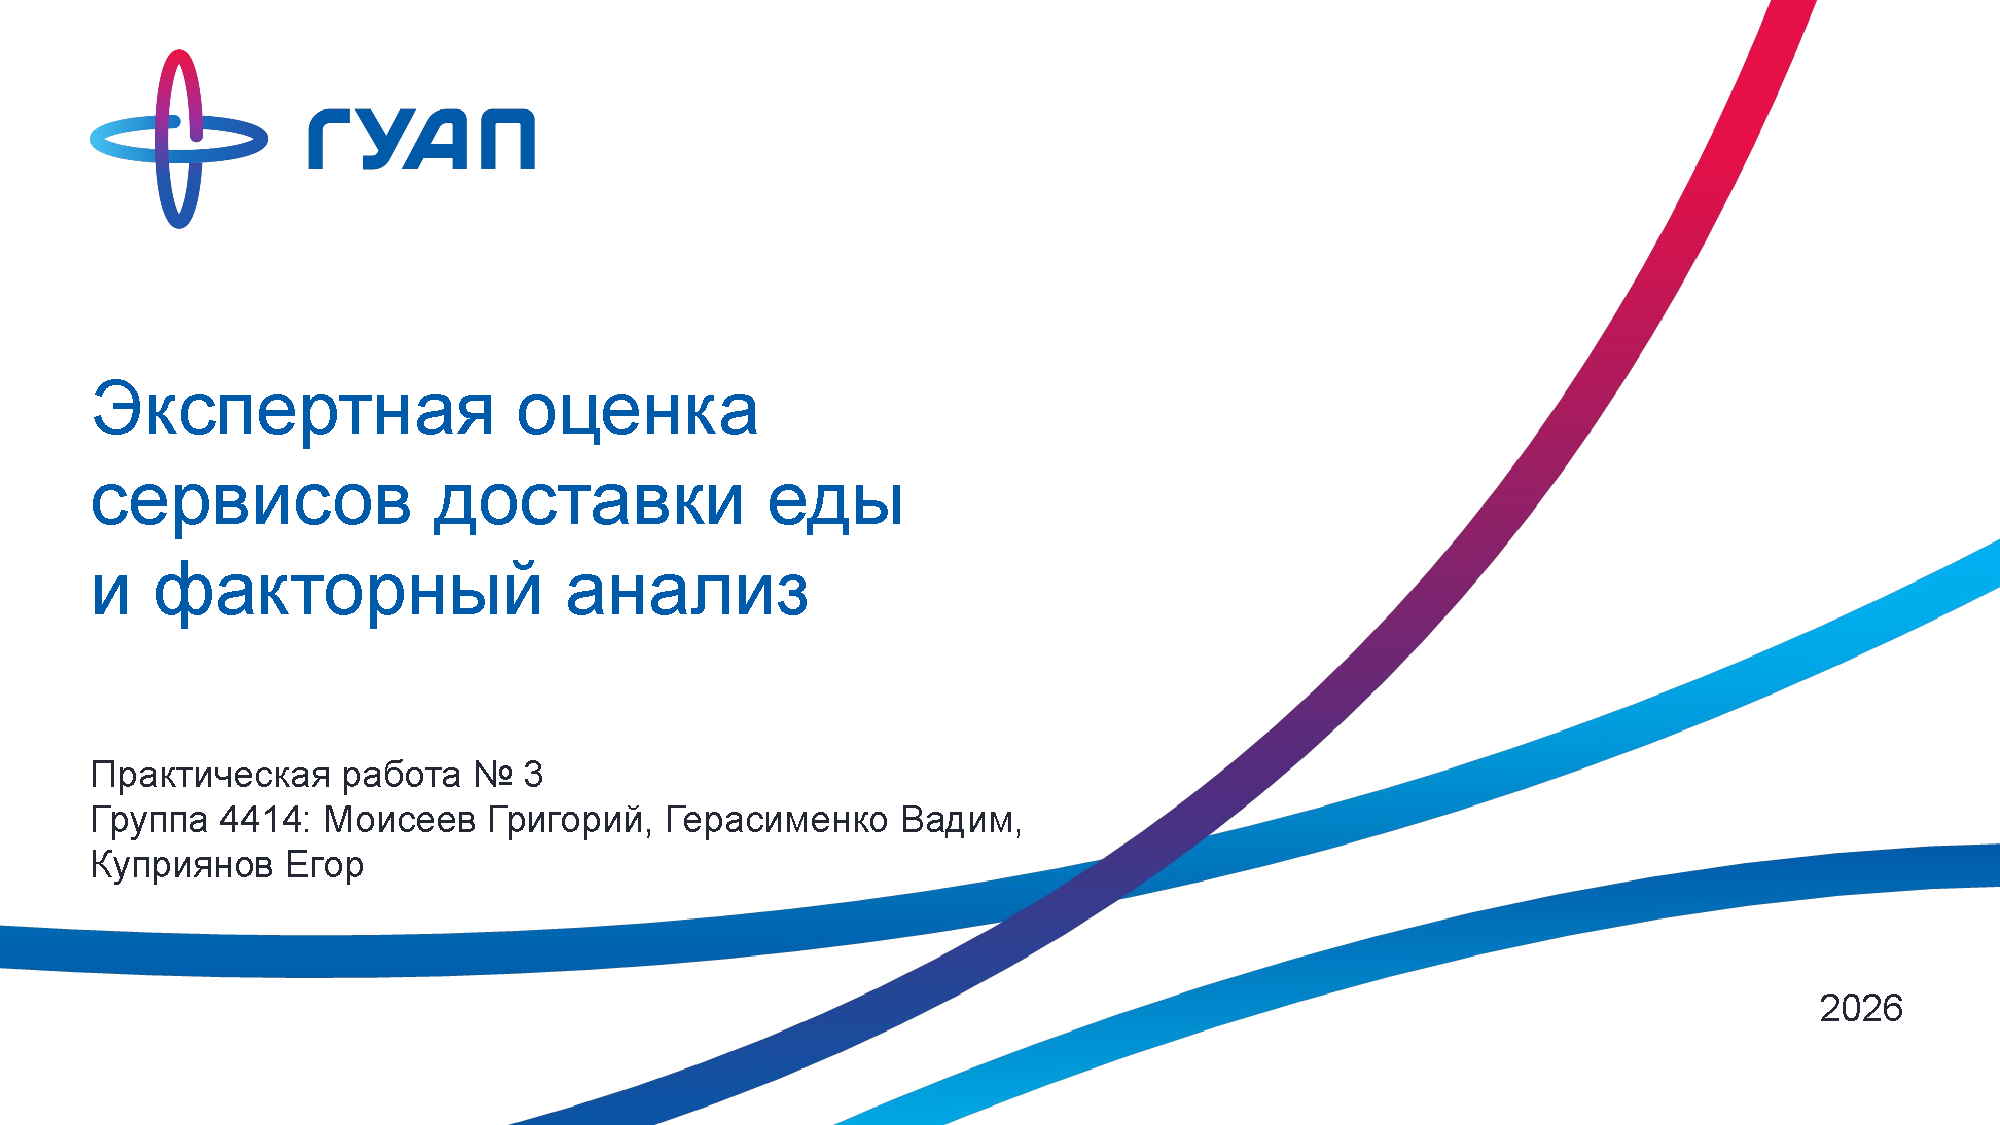
\includepdf[pages=-,pagecommand={},width=0.95\paperwidth]{generated/Presentation.pdf}


\gostappendix{Г}{Электронные материалы к отчету}

Электронная версия материалов размещена в репозитории проекта. В таблице Г.1 приведены ссылки на основные файлы, которые использовались при подготовке расчётов, отчёта и презентации.

\begin{table}[H]
\centering
\caption{Электронные материалы, приложенные к отчету}
\label{tab:digital_appendix}
{\small
\setlength{\tabcolsep}{3.2pt}
\renewcommand{\arraystretch}{1.18}
\begin{tabular}{L{4.6cm}L{5.6cm}L{3.3cm}}
\toprule
Файл или папка & Назначение & Ссылка \\
\midrule
Презентация & PPTX-файл презентации с результатами исследования. & \href{https://github.com/Echways/SPoI/blob/main/lab-3/presentation/Presentation.pptx}{\texttt{открыть pptx}} \\
Код анализа & Jupyter Notebook, в котором выполнены предобработка, факторный анализ, критерий Фридмана, регрессия, построение графиков и таблиц. & \href{https://github.com/Echways/SPoI/blob/main/lab-3/src/jupyter.ipynb}{\texttt{открыть ipynb}} \\
Графики & Графики, использованные в отчёте и презентации. & \href{https://github.com/Echways/SPoI/tree/main/lab-3/assets}{\texttt{открыть папку}} \\
CSV-таблицы & Таблицы с результатами расчётов и очищенной матрицей ответов. & \href{https://github.com/Echways/SPoI/tree/main/lab-3/tables}{\texttt{открыть папку}} \\
Исходные ответы & Исходный файл анкетирования, на основе которого выполнен анализ. & \href{https://github.com/Echways/SPoI/blob/main/lab-3/data/otvety.xlsx}{\texttt{открыть xlsx}} \\
\bottomrule
\end{tabular}}
\end{table}

\end{document}